\chapter{Numerical Experiments}\label{chap: experiments}

In previous sections, we derived a general framework for classification at the top and showed that multiple well-known formulations fall into it. The summary of all formulations presented in this work is available in Table~\ref{tab: summary formulations}. The goal of this chapter is to verify the properties of these formulations experimentally.

\section{Settings}\label{sec: settings}

In this section, we describe in detail all settings used for the experiments. The section consists of five subsections. The first one discusses which formulations from Table~\ref{tab: summary formulations} we use for the experimental evaluation. In this subsection, we also introduce baseline formulations used for the comparison. In the second one, we introduce datasets used in the experiments and describe their structure. A detailed description of the datasets is then provided in separate sections with their corresponding experiment results. The third and fourth subsections contain a detailed description of performance metrics. The last subsection contains a description of tools used for implementation. All codes used for the experiments, as well as all experiment configurations, are publicly available on GitHub:
\begin{center}
  \url{https://github.com/VaclavMacha/ClassificationAtTopExperiments.jl}
\end{center}

\subsection{Formulations}

Formulations from Table~\ref{tab: summary formulations} can be divided into three categories:
\begin{itemize}
  \item The first category contains \TopPush and \TopPushK formulations. These formulations minimize the surrogate approximation of the false-negative rate and use the mean of a small fraction of the negative samples with the highest scores as a threshold.
  \item The second category consists of \Grill, \TopMeanK, and \PatMat formulations. Similarly to \TopPush and \TopPushK, these formulations use the surrogate approximation of the false-negative rate as an objective function. The \Grill formulation also adds the surrogate approximation of the false-positive rate into the objective function. All three formulations use some approximation of the top $\tau$-quantile of all scores as a threshold.
  \item The last category consists of \GrillNP, \tauFPL, and \PatMatNP. These formulations use the same objectives as their corresponding formulations from the second category. However, they differ in the definition of the decision threshold. All three formulations use some kind of approximation of the top $\tau$-quantile of negative scores as a threshold.
\end{itemize}
To simplify the setup of all experiments, we decided to focus on formulations that only use negative samples for the threshold computation, i.e., formulations from the first and third categories. Moreover, we decided to omit the \GrillNP formulation in the final experiments because of its poor results in preliminary experiments. The performance of selected formulations can be compared by basic performance metrics, as shown later in Section~\ref{sec: performance criteria}.

In total, we use four different formulations from Table~\ref{tab: summary formulations}, namely \TopPush, \TopPushK, \tauFPL, and \PatMatNP. Moreover, for \TopPushK, we use two different values of~$K = \{5, 10\}$ and consider the resulting formulations as separate formulations, i.e., we have \TopPushK(5) and \TopPushK(10). Similarly, for \tauFPL and \PatMat we use two different values of~$\tau = \{0.01, 0.05\}.$ For all formulations, we use the hinge loss defined in Notation~\ref{not: surrogates} as a surrogate function.

The final number of unique formulations is seven. To show that they bring advantages, we must compare them to standard methods. In previous chapters, we showed how to solve presented formulations in their primal (Chapters~\ref{chap: linear} and~\ref{chap: deep}) and dual form (Chapter~\ref{chap: dual}). Whenever we use the primal form in the experiments, we use binary cross-entropy defined in the following way as a baseline formulation
\begin{mini}{\bm{w}}{
  \frac{1}{\nall} \sum_{i \in \I} \Brac{- y_i \log(s_i) - (1 - y_i) \log (1 - s_i)}
  }{\label{eq: crossentropy}}{}
  \addConstraint{s_i}{= f(\bm{x}_i; \bm{w}), \quad i \in \I.}
\end{mini}
We decided to use binary cross-entropy since it is one of the most used objective functions for binary classification in machine learning applications. We will denote binary cross-entropy in the following text as \BaseLine. In experiments with dual forms of our formulations, we use C-SVC variant of SVM~\cite{boser1992training, cortes1995support,chang2011libsvm} defined by
\begin{mini}{\bm{w}, b, \bm{\xi}}{
  \frac{1}{2} \norm{\bm{w}}^2 + C \sum_{i \in \I} \xi_i
  }{\label{eq: SVM}}{}
  \addConstraint{y_i}{\Brac{\bm{w}^{\top} \phi(\bm{x}_i) + b} \geq 1 - \xi_i, \quad i \in \I}
  \addConstraint{\xi_i}{\geq 0, \quad i \in \I,}
\end{mini}
where~$y_i \in \{-1, 1\}$ for all~$i \in \I$ and~$\phi(\bm{x}_i)$ maps~$\bm{x}_i$ into a higher-dimensional space (see Section~\ref{sec: kernels}). The corresponding dual form is as follows
\begin{maxi}{\bm{\alpha}}{
  - \frac{1}{2} \bm{\alpha}^{\top} \K \bm{\alpha} - \sum_{i = 1}^{\nall} \alpha_i
  }{\label{eq: SVM dual}}{}
  \addConstraint{\sum_{i = 1}^{\nall} y_i \alpha_i}{= 0}
  \addConstraint{0 \leq \alpha_i }{\leq C, \quad i = 1, 2, \ldots, \nall,}
\end{maxi}
where the kernel matrix~$\K$ is defined for all~$i, j = 1, 2, \ldots, \nall$ as
\begin{equation*}
  \K_{i,j} = y_i y_j k(\bm{x}_i, \bm{x}_j) = \phi(\bm{x}_i)^{\top} \phi(\bm{x}_j).
\end{equation*}
Note that the dual form of C-SVC is very similar to the dual forms of our formulations derived in Chapter~\ref{chap: dual}. We will denote C-SVC as \SVM.

In total, we have nine different formulations for experiments, as seen in Table~\ref{tab: formulations experiments summary}. \BaseLine formulation is used only for experiments with primal forms of our formulations, while \SVM is used only when dual forms are used. The following section discusses which hyper-parameters are used for each formulation. Since we used a slightly different primal form (standard formulation for SVM) for the derivation of dual forms, we also show how to convert used parameters to the resulting dual forms and get identical experiment settings.

\pagebreak

\subsection{Hyperparameters}

The selected formulations differ in the number of available hyper-parameters. Therefore, we decided to use a fixed value for all but one of the hyper-parameters for each formulation. We then use six different values for the remaining non-fixed hyper-parameter to fine-tune the formulation. For most of the considered formulations, the only hyper-parameter is the regularization constant~$\lambda$. The only exceptions are the formulations derived from \PatMatNP since they also have the scaling parameter~$\vartheta.$ Therefore, we use the following six values of this hyper-parameter
\begin{equation*}
  \lambda \in \Brac[c]{10^{-5}, 10^{-4}, 10^{-3}, 10^{-2}, 10^{-1}, 1}
\end{equation*}
for all formulations except \PatMatNP. For formulations derived from \PatMatNP, we fixed~$\lambda$ to~$10^{-3}$ and use the following six different values of the scaling parameter
\begin{equation*}
  \vartheta \in \Brac[c]{10^{-5}, 10^{-4}, 10^{-3}, 10^{-2}, 10^{-1}, 1}.
\end{equation*}
Since we used a slightly different (but equivalent) primal formulation for the derivation of the dual forms, we use~$\lambda$ to compute the hyper-parameter~$C$ used in these dual forms
\begin{equation*}
  C = \frac{1}{\lambda \ntil},
\end{equation*}
where~$\ntil = \nall$ for \SVM and~$\ntil = \npos$ otherwise. In all experiments, the best hyperparameter is selected based on the validation data and the appropriate performance metric. A summary of all used formulations and their hyper-parameters is in Table~\ref{tab: formulations experiments summary}.

\begin{table}[!ht]
  \centering
  \begin{NiceTabular}{lcccc}
    \CodeBefore
      \rowcolor{\headercol}{1}
      \rowcolors{3}{\rowcol}{}[restart]
    \Body
    \toprule
    \textbf{Formulation}
      & \textbf{Fixed parameters}
      & \textbf{Hyper-parameter}
      & \textbf{Primal Form}
      & \textbf{Dual Form} \\
    \midrule
    \BaseLine
      & ---
      & $\lambda$
      & \yesmark
      & \nomark \\
    \SVM
      & ---
      & $\lambda$
      & \nomark 
      & \yesmark \\
    \midrule
    \TopPush
      & ---
      & $\lambda$
      & \yesmark
      & \yesmark \\
    \TopPushK(5)
      & $K = 5$
      & $\lambda$
      & \yesmark
      & \yesmark \\
    \TopPushK(10)
      & $K = 10$
      & $\lambda$
      & \yesmark
      & \yesmark \\
    \tauFPL(0.01)
      & $\tau = 0.01$
      & $\lambda$
      & \yesmark
      & \yesmark \\
    \tauFPL(0.05)
      & $\tau = 0.05$
      & $\lambda$
      & \yesmark
      & \yesmark \\
    \PatMatNP(0.01)
      & $\tau = 0.01,$ $\lambda = 0.001$
      & $\vartheta$
      & \yesmark
      & \yesmark \\
    \PatMatNP(0.05)
      & $\tau = 0.05,$ $\lambda = 0.001$
      & $\vartheta$
      & \yesmark
      & \yesmark \\
    \bottomrule
  \end{NiceTabular}
  \caption{Summary of all formulations used for experiments. The first column shows the aliases used for the formulations when describing the experiment results. The second column shows fixed hyperparameters used for each formulation, while the third column shows which hyper-parameters are tuned using validation data. The last two columns indicate whether the formulation is used in the experiments with primal forms, dual forms, or both.}
  \label{tab: formulations experiments summary}
\end{table}

\pagebreak

\subsection{Datasets}

We consider various datasets summarized in Table~\ref{tab: datasets summary} for the numerical experiments. All these datasets can be divided into three categories:
\begin{enumerate}
  \item \textbf{Image Recognition:} In this category, we test formulations from Table~\ref{tab: formulations experiments summary} on datasets from the domain of image recognition. We use this domain since it is one of the most popular with plenty of publicly available datasets.
  \item \textbf{Steganalysis:} In this category, we use selected formulations in the domain of steganalysis. In this domain, the problem of maximizing the true-positive rate at the specific level of the false-positive rate is well-known and essential, as we show at the beginning of Section~\ref{sec: steganalysis}.
  \item \textbf{Malware Detection:} In this category, we use selected formulations for malware detection. Like in steganalysis, maximizing the true-positive rate at the specific level of the false-positive rate is crucial for malware detection, as discussed at the beginning of Section~\ref{sec: malware detection}.
\end{enumerate}
Each category has a separate section later in the text. It is worth mentioning that not all datasets used in the experiments are primarily designed for the classification at the top. For example, all datasets from the first category are general-purpose image classification datasets. We use these datasets since they are publicly available and well-known. Since all these datasets are multi-class, we need to adjust the labels to get binary classification problems. Therefore, for each data set, we select one class as the positive class and consider the rest as the negative class. 

\begin{table}[!ht]
  \centering
  \resizebox{\columnwidth}{!}{%
    \begin{NiceTabular}{lccrrrrrr}
      \CodeBefore
      \rowcolor{\headercol}{1-2}
      \rowcolors{4}{\rowcol}{}[restart]
      \Body
      \toprule
      \Block[c]{2-1}{\textbf{Dataset}}
      & \Block[c]{2-1}{$y^+$}
      & \Block[c]{2-1}{$d$}
      & \Block[c]{1-2}{\textbf{Train}}
      && \Block[c]{1-2}{\textbf{Validation}}
      && \Block[c]{1-2}{\textbf{Test}} \\
      \cline{4-9}
      &&& \Block[c]{1-1}{$n$}
      & \Block[c]{1-1}{$\frac{\npos}{n}$}
      & \Block[c]{1-1}{$n$}
      & \Block[c]{1-1}{$\frac{\npos}{n}$}
      & \Block[c]{1-1}{$n$}
      & \Block[c]{1-1}{$\frac{\npos}{n}$} \\
      \midrule
      MNIST
      & 1
      & $28 \times 28 \times 1$
      & 45 000
      & 11.3\%
      & 15 000
      & 11.2\%
      & 10 000
      & 11.4\% \\
      FashionMNIST
      & 1
      & $28 \times 28\times 1$
      & 45 000
      & 10.0\%
      & 15 000
      & 9.9\%
      & 10 000
      & 10.0\% \\
      CIFAR10
      & 1
      & $32 \times 32 \times 3$
      & 37 500
      & 10.0\%
      & 12 500
      & 9.9\%
      & 10 000
      & 10.0\% \\
      CIFAR20
      & 1
      & $32 \times 32 \times 3$
      & 37 500
      & 5.0\%
      & 12 500
      & 5.1\%
      & 10 000
      & 5.0\% \\
      CIFAR100
      & 1
      & $32 \times 32 \times 3$
      & 37 500
      & 1.0\%
      & 12 500
      & 1.0\%
      & 10 000
      & 1.0\% \\
      SVHN2
      & 1
      & $32 \times 32\times 3$
      & 54 944
      & 18.9\%
      & 18 313
      & 18.9\%
      & 26 032
      & 19.6\% \\
      SVHN2-Extra
      & 1
      & $32 \times 32\times 3$
      & 453 291
      & 17.3\%
      & 151 097
      & 17.1\%
      & 26 032
      & 19.6\% \\
      \midrule
      \bad{Nsf5}
      & ---
      & $22 510 \times 1$
      & 186 583
      & 9.1\%
      & 62 194
      & 9.1\%
      & 248 776
      & 9.1\% \\
      \bad{JMiPOD}
      & ---
      & $256 \times 256\times 3$
      & 186 515
      & 9.1\%
      & 62 172
      & 9.1\%
      & 248 686
      & 9.1\% \\
      \midrule
      \bad{Malware}
      & ---
      & variable
      & 6 580 166
      & 87.22\%
      & ---
      & ---
      & 800 346
      & 91.8\% \\
      \bottomrule
    \end{NiceTabular}
  }
  \caption{Structure of datasets: The training, validation and testing sets show the positive label~$y^+,$ the number of features~$d$, samples~$n$ and the fraction of positive samples~$\frac{\npos}{n}$. Datasets depicted in red are not publicly available.}
  \label{tab: datasets summary}
\end{table}

\subsection{Performance Criteria}\label{sec: performance criteria}

In this section, we describe which performance criteria are used for evaluation and how these criteria are related to the tested formulations.

As we discussed at the beginning of Section~\ref{sec: settings}, we decided to only test formulations that minimize the false-negative rate (or a combination of false-negative and false-positive rate) and use only negative samples for the threshold computation. This choice allows us to use simple metrics to compare the formulations. The first metric that we use in the experiments is~$\tpratk$ defined as follows
\begin{equation*}
  \tpratk = \frac{1}{\npos} \sum_{i \in \Ipos} \Iverson{s_i \geq t} \quad \text{where} \quad t = \frac{1}{K} \sum_{j = 1}^{K} s^{-}_{[j]}.
\end{equation*}
This metric computes the true-positive rate at a threshold~$t$ defined as the mean of $K$-largest negative scores. For~$K = 1$, the threshold corresponds to the threshold used by \TopPush formulation. Otherwise, threshold~$t$ corresponds to the threshold used by \TopPushK. Moreover, since minimizing the false-negative rate is equivalent to maximizing the true-positive rate, both \TopPush and \TopPushK should optimize the $\tpratk$ metric. In the upcoming experiments, we use this metric with three different values of~$K \in \{1, 5, 10\}.$

The second metric is defined in a similar way
\begin{equation*}
  \tpratfpr = \frac{1}{\npos} \sum_{i \in \Ipos} \Iverson{s_i \geq t} \quad \text{where} \quad t
  = \max \Set{t}{\frac{1}{\nneg} \sum_{i \in \Ineg} \Iverson{s_i \geq t} \geq \tau}.
\end{equation*}
This metric computes the true-positive rate at a specific top $\tau$-quantile of negative scores. This metric is ideal for testing the performance of \tauFPL and \PatMatNP formulations since both maximize the true-positive rate and use some approximation of the true top $\tau$-quantile of negative scores as a threshold. In our experiments, we use this metric with two different values of~$\tau \in \{0.01, 0.05\}.$

The two previous metrics are specific to the formulations from our framework. However, we should also test if the baseline formulations work correctly. Since the baseline methods are designed to optimize overall performance, we use the area under the ROC curve to measure the overall performance. The summary of all used metrics is in Table~\ref{tab: metrics summary}.

\begin{table}[!ht]
  \centering
  \begin{NiceTabular}{lcccccc}
    \CodeBefore
    \rowcolor{\headercol}{1-2}
    \rowcolors{4}{\rowcol}{}[restart]
    \Body
    \toprule
    \Block[c]{2-1}{\textbf{Formulation}}
      & \Block[c]{2-1}{$\auroc$}
      & \Block[c]{1-3}{$\tpratk$}
      &&& \Block[c]{1-2}{$\tpratfpr$} \\
    \cline{3-7}
      && $1$  
      & $5$
      & $10$
      & $0.01$
      & $0.05$ \\
    \midrule
    \BaseLine
      & \yesmark
      & \nomark
      & \nomark
      & \nomark
      & \nomark
      & \nomark \\
    \SVM
      & \yesmark
      & \nomark
      & \nomark
      & \nomark
      & \nomark
      & \nomark \\
    \midrule
    \TopPush
      & \nomark
      & \yesmark
      & \nomark
      & \nomark
      & \nomark
      & \nomark \\
    \TopPushK(5)
      & \nomark
      & \nomark
      & \yesmark
      & \nomark
      & \nomark
      & \nomark \\
    \TopPushK(10)
      & \nomark
      & \nomark
      & \nomark
      & \yesmark
      & \nomark
      & \nomark \\
    \tauFPL(0.01) and \PatMatNP(0.01)
      & \nomark
      & \nomark
      & \nomark
      & \nomark
      & \yesmark
      & \nomark \\
    \tauFPL(0.05) and \PatMatNP(0.05)
      & \nomark
      & \nomark
      & \nomark
      & \nomark
      & \nomark
      & \yesmark \\
    \bottomrule
  \end{NiceTabular}
  \caption{The summary of all used performance metrics used for evaluation. In total, we use six different metrics and nine different formulations. For each formulation~\yesmark denotes the metric in which the formulation should be the best.}
  \label{tab: metrics summary}
\end{table}

\subsection{Critical Difference Diagrams}\label{sec: cd evaluation}

All metrics from Section~\ref{sec: performance criteria} can be used to compare different formulations on a single dataset. However, these metrics are unsuitable for comparing multiple formulations on multiple datasets. To address this issue, we use the Friedman test~\cite{friedman1940comparison} as suggested in~\cite{demvsar2006statistical}.

Consider that we have~$m$ datasets, and~$k$ formulations. Then for each dataset~$i$, each formulation~$j$ is ranked by rank~$r^i_j$ according to some performance criterium. Any performance metric from the previous section can be used. The formulation that provides the best result gets ranked 1; the second best gets ranked 2, and so on. If two formulations provide the same results, the average ranks are assigned. The average rank overall dataset for formulation~$j$ is computed as
\begin{equation*}
  R_j = \frac{1}{m} \sum_{i = 1}^{m} r^{i}_{j}.
\end{equation*}
The Friedman test compares the average ranks of formulations under the null hypothesis, which states that all formulations are equivalent. Therefore, their average ranks should be equal. If the null hypothesis is rejected, we proceed with the post hoc Nemenyi test~\cite{nemenyi1963distribution} that compares all formulations to each other. The performance of the two formulations is significantly different if the corresponding average
ranks differ by at least the critical difference
\begin{equation*}
  CD = q_{\alpha} \sqrt{\frac{k(k + 1)}{6m}},
\end{equation*}
where critical values~$q_{\alpha}$ are based on the Studentized range statistic divided by~$\sqrt{2},$ see Table 5(a) in~\cite{demvsar2006statistical}. The results of this post hoc test can be easily visualized using critical difference diagrams proposed in~\cite{demvsar2006statistical}. The $x$-axis of such a diagram shows the average rank over all datasets for each formulation. Formulations that are not significantly different according to the Nemenyi test are connected using a green horizontal line. As an example, see Figure~\ref{fig: primal linear CD}.

\subsection{Implementation}

For the implementation of all experiments, we use the Julia programming language~\cite{bezanson2017julia}. The dual formulations are implemented from scratch, while the primal formulations are implemented using Flux.jl~\cite{innes:2018, Flux.jl-2018} library. This library provides all the necessary tools for building neural networks. Moreover, the library allows the implementation of a custom gradient for any function, which allows us to implement all formulations from Table~\ref{tab: summary formulations}. For experiments with SVM, we use the Julia wrapper for the LIBSVM library~\cite{chang2011libsvm}.

\section{Image Recognition}\label{sec: image recognition}

In this section, we present experiments with six well-known image recognition datasets. All these datasets are publicly available. MNIST~\cite{deng2012mnist} and FashionMNIST~\cite{xiao2017fashionmnist} are grayscale datasets of digits and fashion items, respectively. CIFAR100~\cite{krizhevsky2009learning} is a dataset of colored images of different items grouped into 100 classes. CIFAR10 and CIFAR20 merge these classes into 10 and 20 superclasses, respectively. Finally, SVHN2~\cite{netzer2011reading} contains colored images of house numbers. All these datasets are originally divided only into training and test sets. We select 25\% samples from the training set to obtain the validation set. For a more detailed description of the structure of datasets, see Table~\ref{tab: datasets summary}.

None of these datasets are primarily designed for the problem of classification at the top. We presented these datasets to show that introduced formulations can be helpful even for general-purpose datasets and may improve performance on specific metrics. However, there are some drawbacks to using these datasets. For example, many state-of-the-art neural network architectures achieve almost the perfect classification on some of these datasets. Therefore, there is no room for improvement, and we have to use much simpler architectures to show the behavior of formulations presented in this work (Section~\ref{sec: results primal nonlinear}).

For comparison we use critical difference diagrams introduced in Section~\ref{sec: cd evaluation}. One of the basic assumptions of the critical difference diagrams to work appropriately is a large number of used datasets. Since we performed all experiments for each formulation and each dataset ten times with different random seeds for train/valid/test split, we decided to consider each of these runs as a separate dataset. It is important to say that we use this setting only for the critical difference diagrams. Since the critical diagrams show the relative performance of the formulations against each other, we can easily see if any formulation is significantly worse or better. However, the critical diagrams do not provide any information on the actual performance of the formulations. Therefore, even if one formulation outperforms other tested formulations, it does not mean that its performance is good.

To address the issue above, we also compare concrete performance metrics on each dataset separately. Since we have six hyperparameters for each formulation, we always select the best result for each formulation on the validation set based on the criterion for which the specific formulation is optimized. Then for each formulation, we select the median of the best results from ten independent runs. Moreover, the best result for each dataset is highlighted in green, while the worst result is highlighted in red.


\subsection{Primal Formulation: Linear Model}\label{sec: results primal linear}

In this section, we present results for a primal form of formulations from Table~\ref{tab: formulations experiments summary} with a linear model. For training, we use stochastic gradient descent with balanced mini-batches of size 512. As an optimizer, we use the ADAM~\cite{kingma2014adam} with default settings and initial step length~$\alpha = 0.01$, which we discount every five epochs by the factor of~$0.8$ using an exponential decay scheme. We also fix the number of epochs to 100, and repeat each experiment ten times with different random seeds.

As mentioned earlier, we use critical difference diagrams (Figure~\ref{fig: primal linear CD}) and medians of ten independent runs (Table~\ref{tab: primal linear medians}) for comparison. We make several observations:
\begin{itemize}
  \item \TopPushK formulations provide a slight (not statistically significant) improvement over \TopPush in most of the experiments, as shown in Figure~\ref{fig: primal linear CD}, where a green line connects all three formulations for almost all metrics. The only exception is the $\tpratfpr=0.01$ metric, for which \TopPush is significantly worse than other formulations.
  \item \BaseLine formulation works best for $\auroc$ metric and is not suitable for any other metric; see Figure~\ref{fig: primal linear CD} or Table~\ref{tab: primal linear medians}. \BaseLine consistently provides the best results for $\auroc$ for all datasets. On the other hand, \BaseLine works poorly for metrics that operate at the absolute top, such as~$\tpratk = 1,$~$\tpratk = 5,$ or $\tpratk = 10.$
  \item \PatMatNP formulations provide very good results for all metrics. Moreover, \PatMatNP(0.01) is the best formulation for $\tpratfpr = 0.01,$ and \PatMatNP(0.05) for $\tpratfpr = 0.05.$ It means that both methods are the best for the criterion for which they are optimized. The same behavior can also be seen in Table~\ref{tab: primal linear medians}, where \PatMatNP(0.05) is the best formulation for $\tpratfpr = 0.01$ almost for all datasets.
  \item \tauFPL(0.05) works very well for both $\tpratfpr = 0.01$ and $\tpratfpr = 0.05.$. The formulation achieves almost as good results for both metrics as \PatMatNP formulations.
  \item All formulations provide very poor results for CIFAR and SVHN2 datasets, as shown in Table~\ref{tab: primal linear medians}. The use of a simple linear model causes this. However, the obtained results are still relevant since we compare the relative performance of the formulations to each other and not the absolute performance.
\end{itemize}

\begin{figure}[!p]
  \centering
  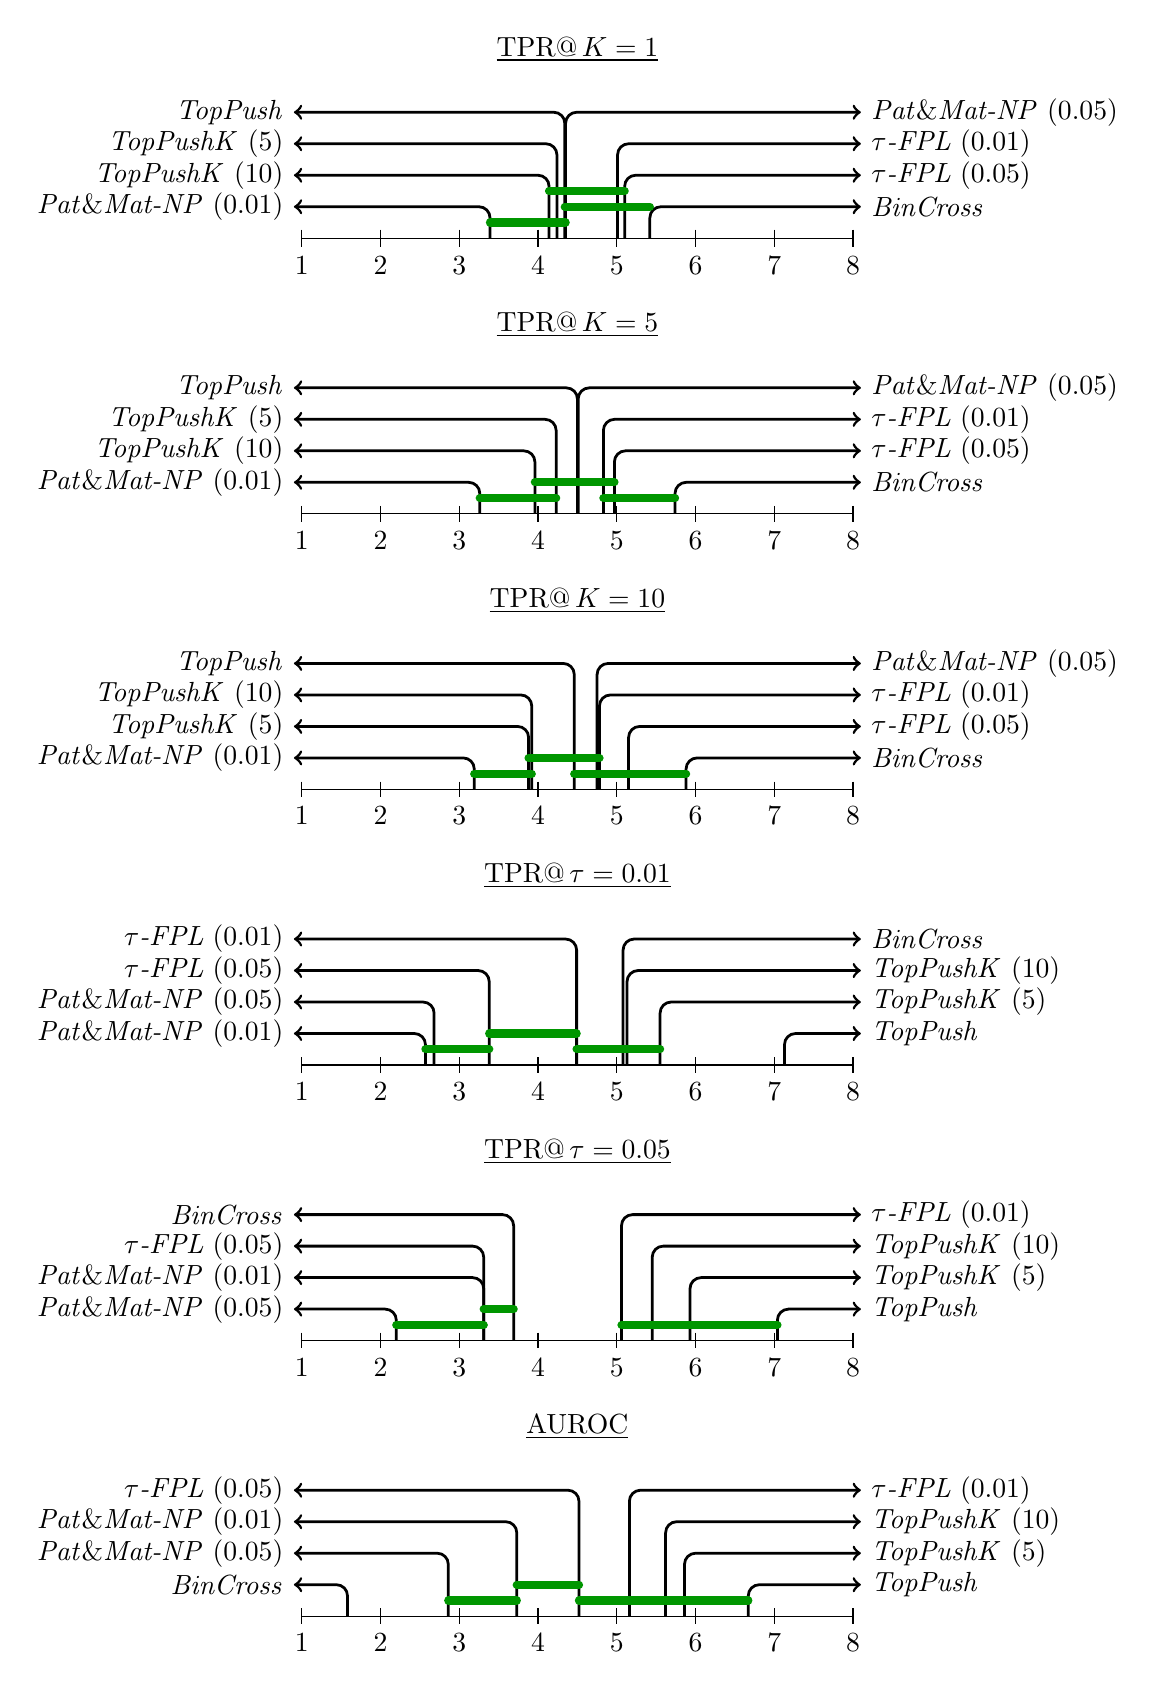
\begin{tikzpicture}  \node at (4.5,2.4) {\underline{$\auroc$}}; 
  \draw (1,0) -- (8,0); 
  \foreach \x in {1,...,8} \draw (\x,0.1) -- (\x,-0.1) node[anchor=north]{$\x$}; 
  \draw[line_node] (1.58,0) -- (1.58,0.4) -- (0.9, 0.4) node[anchor=east] {\BaseLine}; 
  \draw[line_node] (2.86,0) -- (2.86,0.8) -- (0.9, 0.8) node[anchor=east] {\PatMatNP(0.05)}; 
  \draw[line_node] (3.73,0) -- (3.73,1.2) -- (0.9, 1.2) node[anchor=east] {\PatMatNP(0.01)}; 
  \draw[line_node] (4.52,0) -- (4.52,1.6) -- (0.9, 1.6) node[anchor=east] {\tauFPL(0.05)}; 
  \draw[line_node] (5.16,0) -- (5.16,1.6) -- (8.1, 1.6) node[anchor=west] {\tauFPL(0.01)}; 
  \draw[line_node] (5.62,0) -- (5.62,1.2) -- (8.1, 1.2) node[anchor=west] {\TopPushK(10)}; 
  \draw[line_node] (5.86,0) -- (5.86,0.8) -- (8.1, 0.8) node[anchor=west] {\TopPushK(5)}; 
  \draw[line_node] (6.67,0) -- (6.67,0.4) -- (8.1, 0.4) node[anchor=west] {\TopPush}; 
  \draw[line_cv] (2.86,0.2) -- (3.73, 0.2); 
  \draw[line_cv] (3.73,0.4) -- (4.52, 0.4); 
  \draw[line_cv] (4.52,0.2) -- (5.62, 0.2); 
  \draw[line_cv] (5.16,0.2) -- (5.86, 0.2); 
  \draw[line_cv] (5.62,0.2) -- (6.67, 0.2); 


  \node at (4.5,5.9) {\underline{$\tpratfpr = 0.05$}}; 
  \draw (1,3.5) -- (8,3.5); 
  \foreach \x in {1,...,8} \draw (\x,3.6) -- (\x,3.4) node[anchor=north]{$\x$}; 
  \draw[line_node] (2.2,3.5) -- (2.2,3.9) -- (0.9, 3.9) node[anchor=east] {\PatMatNP(0.05)}; 
  \draw[line_node] (3.31,3.5) -- (3.31,4.3) -- (0.9, 4.3) node[anchor=east] {\PatMatNP(0.01)}; 
  \draw[line_node] (3.31,3.5) -- (3.31,4.7) -- (0.9, 4.7) node[anchor=east] {\tauFPL(0.05)}; 
  \draw[line_node] (3.69,3.5) -- (3.69,5.1) -- (0.9, 5.1) node[anchor=east] {\BaseLine}; 
  \draw[line_node] (5.06,3.5) -- (5.06,5.1) -- (8.1, 5.1) node[anchor=west] {\tauFPL(0.01)}; 
  \draw[line_node] (5.45,3.5) -- (5.45,4.7) -- (8.1, 4.7) node[anchor=west] {\TopPushK(10)}; 
  \draw[line_node] (5.93,3.5) -- (5.93,4.3) -- (8.1, 4.3) node[anchor=west] {\TopPushK(5)}; 
  \draw[line_node] (7.04,3.5) -- (7.04,3.9) -- (8.1, 3.9) node[anchor=west] {\TopPush}; 
  \draw[line_cv] (2.2,3.7) -- (3.31, 3.7); 
  \draw[line_cv] (3.31,3.9) -- (3.69, 3.9); 
  \draw[line_cv] (5.06,3.7) -- (5.93, 3.7); 
  \draw[line_cv] (5.93,3.7) -- (7.04, 3.7); 


  \node at (4.5,9.4) {\underline{$\tpratfpr = 0.01$}}; 
  \draw (1,7.0) -- (8,7.0); 
  \foreach \x in {1,...,8} \draw (\x,7.1) -- (\x,6.9) node[anchor=north]{$\x$}; 
  \draw[line_node] (2.57,7.0) -- (2.57,7.4) -- (0.9, 7.4) node[anchor=east] {\PatMatNP(0.01)}; 
  \draw[line_node] (2.68,7.0) -- (2.68,7.8) -- (0.9, 7.8) node[anchor=east] {\PatMatNP(0.05)}; 
  \draw[line_node] (3.38,7.0) -- (3.38,8.2) -- (0.9, 8.2) node[anchor=east] {\tauFPL(0.05)}; 
  \draw[line_node] (4.49,7.0) -- (4.49,8.6) -- (0.9, 8.6) node[anchor=east] {\tauFPL(0.01)}; 
  \draw[line_node] (5.08,7.0) -- (5.08,8.6) -- (8.1, 8.6) node[anchor=west] {\BaseLine}; 
  \draw[line_node] (5.13,7.0) -- (5.13,8.2) -- (8.1, 8.2) node[anchor=west] {\TopPushK(10)}; 
  \draw[line_node] (5.55,7.0) -- (5.55,7.8) -- (8.1, 7.8) node[anchor=west] {\TopPushK(5)}; 
  \draw[line_node] (7.13,7.0) -- (7.13,7.4) -- (8.1, 7.4) node[anchor=west] {\TopPush}; 
  \draw[line_cv] (2.57,7.2) -- (3.38, 7.2); 
  \draw[line_cv] (3.38,7.4) -- (4.49, 7.4); 
  \draw[line_cv] (4.49,7.2) -- (5.55, 7.2); 


  \node at (4.5,12.9) {\underline{$\tpratk =10$}}; 
  \draw (1,10.5) -- (8,10.5); 
  \foreach \x in {1,...,8} \draw (\x,10.6) -- (\x,10.4) node[anchor=north]{$\x$}; 
  \draw[line_node] (3.19,10.5) -- (3.19,10.9) -- (0.9, 10.9) node[anchor=east] {\PatMatNP(0.01)}; 
  \draw[line_node] (3.88,10.5) -- (3.88,11.3) -- (0.9, 11.3) node[anchor=east] {\TopPushK(5)}; 
  \draw[line_node] (3.92,10.5) -- (3.92,11.7) -- (0.9, 11.7) node[anchor=east] {\TopPushK(10)}; 
  \draw[line_node] (4.46,10.5) -- (4.46,12.1) -- (0.9, 12.1) node[anchor=east] {\TopPush}; 
  \draw[line_node] (4.75,10.5) -- (4.75,12.1) -- (8.1, 12.1) node[anchor=west] {\PatMatNP(0.05)}; 
  \draw[line_node] (4.78,10.5) -- (4.78,11.7) -- (8.1, 11.7) node[anchor=west] {\tauFPL(0.01)}; 
  \draw[line_node] (5.15,10.5) -- (5.15,11.3) -- (8.1, 11.3) node[anchor=west] {\tauFPL(0.05)}; 
  \draw[line_node] (5.88,10.5) -- (5.88,10.9) -- (8.1, 10.9) node[anchor=west] {\BaseLine}; 
  \draw[line_cv] (3.19,10.7) -- (3.92, 10.7); 
  \draw[line_cv] (3.88,10.9) -- (4.78, 10.9); 
  \draw[line_cv] (4.46,10.7) -- (5.15, 10.7); 
  \draw[line_cv] (4.75,10.7) -- (5.88, 10.7); 


  \node at (4.5,16.4) {\underline{$\tpratk =5$}}; 
  \draw (1,14.0) -- (8,14.0); 
  \foreach \x in {1,...,8} \draw (\x,14.1) -- (\x,13.9) node[anchor=north]{$\x$}; 
  \draw[line_node] (3.26,14.0) -- (3.26,14.4) -- (0.9, 14.4) node[anchor=east] {\PatMatNP(0.01)}; 
  \draw[line_node] (3.96,14.0) -- (3.96,14.8) -- (0.9, 14.8) node[anchor=east] {\TopPushK(10)}; 
  \draw[line_node] (4.23,14.0) -- (4.23,15.2) -- (0.9, 15.2) node[anchor=east] {\TopPushK(5)}; 
  \draw[line_node] (4.5,14.0) -- (4.5,15.6) -- (0.9, 15.6) node[anchor=east] {\TopPush}; 
  \draw[line_node] (4.51,14.0) -- (4.51,15.6) -- (8.1, 15.6) node[anchor=west] {\PatMatNP(0.05)}; 
  \draw[line_node] (4.83,14.0) -- (4.83,15.2) -- (8.1, 15.2) node[anchor=west] {\tauFPL(0.01)}; 
  \draw[line_node] (4.97,14.0) -- (4.97,14.8) -- (8.1, 14.8) node[anchor=west] {\tauFPL(0.05)}; 
  \draw[line_node] (5.74,14.0) -- (5.74,14.4) -- (8.1, 14.4) node[anchor=west] {\BaseLine}; 
  \draw[line_cv] (3.26,14.2) -- (4.23, 14.2); 
  \draw[line_cv] (3.96,14.4) -- (4.97, 14.4); 
  \draw[line_cv] (4.83,14.2) -- (5.74, 14.2); 


  \node at (4.5,19.9) {\underline{$\tpratk =1$}}; 
  \draw (1,17.5) -- (8,17.5); 
  \foreach \x in {1,...,8} \draw (\x,17.61) -- (\x,17.39) node[anchor=north]{$\x$}; 
  \draw[line_node] (3.39,17.5) -- (3.39,17.9) -- (0.9, 17.9) node[anchor=east] {\PatMatNP(0.01)}; 
  \draw[line_node] (4.14,17.5) -- (4.14,18.3) -- (0.9, 18.3) node[anchor=east] {\TopPushK(10)}; 
  \draw[line_node] (4.24,17.5) -- (4.24,18.7) -- (0.9, 18.7) node[anchor=east] {\TopPushK(5)}; 
  \draw[line_node] (4.34,17.5) -- (4.34,19.1) -- (0.9, 19.1) node[anchor=east] {\TopPush}; 
  \draw[line_node] (4.35,17.5) -- (4.35,19.1) -- (8.1, 19.1) node[anchor=west] {\PatMatNP(0.05)}; 
  \draw[line_node] (5.01,17.5) -- (5.01,18.7) -- (8.1, 18.7) node[anchor=west] {\tauFPL(0.01)}; 
  \draw[line_node] (5.1,17.5) -- (5.1,18.3) -- (8.1, 18.3) node[anchor=west] {\tauFPL(0.05)}; 
  \draw[line_node] (5.42,17.5) -- (5.42,17.9) -- (8.1, 17.9) node[anchor=west] {\BaseLine}; 
  \draw[line_cv] (3.39,17.7) -- (4.35, 17.7); 
  \draw[line_cv] (4.14,18.1) -- (5.1, 18.1); 
  \draw[line_cv] (4.34,17.9) -- (5.42, 17.9); 
\end{tikzpicture}

  \caption{\textbf{Primal formulation with a linear model:} Critical difference diagrams (level of importance 0.05) of the Nemenyi post hoc test for the Friedman test. Each diagram shows the mean rank of each method, with rank one being the best. The green horizontal lines group methods with mean ranks that are not significantly different. The critical difference diagrams were computed for mean rank averages over all datasets.}
  \label{fig: primal linear CD}
\end{figure}


\begin{table}[!p]
  \centering
  \underline{$\tpratk =10$}
  \vspace{0.25cm}\\
  \resizebox{\columnwidth}{!}{% 
    \begin{NiceTabular}{lccccccc}
      \CodeBefore
        \rowcolor{\headercol}{1}
        \rowcolors{3}{\rowcol}{}[restart]
      \Body
      \toprule
      \textbf{Formulation}
        & \textbf{MNIST}
        & \textbf{FashionMNIST}
        & \textbf{CIFAR10}
        & \textbf{CIFAR20}
        & \textbf{CIFAR100}
        & \textbf{SVHN2}
        & \textbf{SVHN2Extra}\\
      \midrule
      \BaseLine
        & 68.54
        & 85.65
        & \worst{1.25}
        & \best{1.40}
        & \worst{2.00}
        & 0.04
        & \worst{0.02}\\
      \TopPush
        & 89.38
        & \best{93.70}
        & 2.25
        & \worst{0.40}
        & 4.00
        & \worst{0.02}
        & \worst{0.02}\\
      \TopPushK(5)
        & 89.60
        & 93.30
        & 3.30
        & 1.10
        & 3.00
        & 0.04
        & 0.06\\
      \TopPushK(10)
        & \best{89.64}
        & 92.75
        & 3.90
        & 0.70
        & 4.50
        & 0.04
        & \best{0.09}\\
      \tauFPL(0.01)
        & 83.35
        & 92.40
        & 2.90
        & 0.80
        & 2.50
        & 0.03
        & \worst{0.02}\\
      \tauFPL(0.05)
        & \worst{40.26}
        & \worst{79.65}
        & 3.60
        & 1.00
        & \best{5.50}
        & 0.04
        & \best{0.09}\\
      \PatMatNP(0.01)
        & 87.88
        & 92.75
        & \best{5.00}
        & 1.10
        & 4.00
        & 0.12
        & \best{0.09}\\
      \PatMatNP(0.05)
        & 51.72
        & 81.60
        & 3.80
        & 1.20
        & 3.00
        & \best{0.14}
        & 0.06\\
      \bottomrule
    \end{NiceTabular}
  }
  \vspace{0.25cm}\\
  \underline{$\tpratfpr = 0.05$}
  \vspace{0.25cm}\\
  \resizebox{\columnwidth}{!}{% 
    \begin{NiceTabular}{lccccccc}
      \CodeBefore
        \rowcolor{\headercol}{1}
        \rowcolors{3}{\rowcol}{}[restart]
      \Body
      \toprule
      \textbf{Formulation}
        & \textbf{MNIST}
        & \textbf{FashionMNIST}
        & \textbf{CIFAR10}
        & \textbf{CIFAR20}
        & \textbf{CIFAR100}
        & \textbf{SVHN2}
        & \textbf{SVHN2Extra}\\
      \midrule
      \BaseLine
        & \best{99.65}
        & 99.30
        & 43.40
        & 32.90
        & 54.50
        & 5.53
        & \worst{5.91}\\
      \TopPush
        & \worst{99.12}
        & \worst{98.30}
        & \worst{31.10}
        & \worst{16.30}
        & 43.50
        & \worst{5.22}
        & 6.40\\
      \TopPushK(5)
        & 99.21
        & \worst{98.30}
        & 35.50
        & 20.20
        & \worst{42.50}
        & 6.78
        & 7.42\\
      \TopPushK(10)
        & 99.30
        & \worst{98.30}
        & 37.90
        & 20.80
        & 46.50
        & 6.15
        & 8.07\\
      \tauFPL(0.01)
        & 99.47
        & 98.75
        & 35.85
        & 24.00
        & 44.00
        & 6.90
        & 7.76\\
      \tauFPL(0.05)
        & 99.56
        & 99.20
        & 39.50
        & 25.70
        & 50.50
        & 8.16
        & 9.69\\
      \PatMatNP(0.01)
        & 99.52
        & 98.85
        & 45.35
        & 33.70
        & 56.00
        & 9.28
        & \best{12.47}\\
      \PatMatNP(0.05)
        & \best{99.65}
        & \best{99.40}
        & \best{46.80}
        & \best{34.80}
        & \best{58.50}
        & \best{9.34}
        & 12.25\\
      \bottomrule
    \end{NiceTabular}
  }
  \vspace{0.25cm}\\
  \underline{$\auroc$}
  \vspace{0.25cm}\\
  \centering
  \resizebox{\columnwidth}{!}{% 
    \begin{NiceTabular}{lccccccc}
      \CodeBefore
        \rowcolor{\headercol}{1}
        \rowcolors{3}{\rowcol}{}[restart]
      \Body
      \toprule
      \textbf{Formulation}
        & \textbf{MNIST}
        & \textbf{FashionMNIST}
        & \textbf{CIFAR10}
        & \textbf{CIFAR20}
        & \textbf{CIFAR100}
        & \textbf{SVHN2}
        & \textbf{SVHN2Extra}\\
      \midrule
      \BaseLine
        & \best{99.86}
        & \best{99.83}
        & \best{84.00}
        & \best{76.26}
        & \best{88.48}
        & \best{57.82}
        & \best{56.10}\\
      \TopPush
        & \worst{99.78}
        & \worst{99.42}
        & \worst{73.84}
        & 65.76
        & 82.10
        & 51.08
        & 51.30 \\
      \TopPushK(5)
        & 99.80
        & \worst{99.42}
        & 76.67
        & \worst{65.70}
        & \worst{81.52}
        & \worst{50.98}
        & 50.69\\
      \TopPushK(10)
        & 99.82
        & 99.48
        & 77.74
        & 66.87
        & 81.91
        & 51.90
        & \worst{50.58}\\
      \tauFPL(0.01)
        & 99.84
        & 99.72
        & 77.34
        & 69.24
        & 82.96
        & 51.04
        & 50.62\\
      \tauFPL(0.05)
        & 99.81
        & 99.80
        & 79.41
        & 70.86
        & 84.56
        & 51.78
        & 50.76\\
      \PatMatNP(0.01)
        & 99.85
        & 99.68
        & 82.34
        & 74.56
        & 86.13
        & 56.38
        & 51.93\\
      \PatMatNP(0.05)
        & 99.84
        & 99.81
        & 83.35
        & 75.44
        & 87.22
        & 56.40
        & 52.50\\
      \bottomrule
    \end{NiceTabular}
  }
  \caption{\textbf{Primal formulation with a linear model:} Each table corresponds to one performance metric, and all presented results are medians of ten independent runs for each dataset and formulation pair. The best result for each dataset is highlighted in green, while the worst result is highlighted in red. For better readability, we have reduced the number of discussed metrics compared to Figure~\ref{fig: primal linear CD}.}
  \label{tab: primal linear medians}
\end{table}

\pagebreak

\subsection{Dual Formulation: Linear Model}\label{sec: results dual}

In this section, we present results for a dual form of formulations from Table~\ref{tab: formulations experiments summary} with a Gaussian kernel model. For training, we use the coordinate descent algorithm introduced in Section~\ref{sec: coordinate descent}. We set a number of steps to 20 epochs. For all experiments, we use precomputed kernel matrix with a Gaussian kernel function defined as 
\begin{equation*}
  k(\bm{x}_i, \bm{x}_j) = \exp\Brac[c]{- \frac{\norm{\bm{x}_i - \bm{x}_j}^2}{d}},
\end{equation*}
where~$d$ is the dimension of the primal problem. We used this since it is the default setting for radial basis kernel type in LIBSVM~\cite{chang2011libsvm}.

In Figure~\ref{fig: dual convergence}, we investigate the convergence of the coordinate descend algorithm introduced in Section~\ref{sec: coordinate descent} for three formulations, namely \TopPush, \TopPushK, and \PatMatNP. In each column, we show the primal and dual objective function convergence for one formulation. To solve the primal problem, we used full gradient descent. Computation of the full gradient is computationally intensive, even for relatively small datasets such as MNIST. Therefore, for this experiment (and only for this experiment) we use the Ionosphere dataset~\cite{sigillito1989classification}, which is small. We can see that \TopPush and \TopPushK converge to the same objective for primal and dual problems. It means that both problems were solved to optimality. However, there is a little gap between the optimal primal and dual form solution for \PatMatNP. In other words, \PatMatNP may suffer from convergence issues when solving the proposed coordinate descent algorithm.  

For comparison of all formulations, we use the same two approaches as in Section~\ref{sec: results primal linear}. From Figure~\ref{fig: dual gauss CD} and Table~\ref{tab: dual gauss medians}, we make several observations:
\begin{itemize}
  \item We observe that some formulations have problems with convergence and, in some cases, even diverge for some datasets. The improper choice of the kernel function parameters can be the cause. As a result, CD diagrams may provide unreliable results. If the formulation diverges in some experiments, it immediately obtains very high ranks for these experiments that skew the final diagram. It is especially evident for \PatMatNP and \SVM formulations.
  \item Figure~\ref{fig: dual gauss CD} shows that \PatMatNP formulations provide the worst results for all metrics. It can be caused by the bad convergence of the coordinate descent algorithm, as shown in Figure~\ref{fig: dual convergence}. However, it is important to say that Figure~\ref{fig: dual gauss CD} shows only relative results. From Table~\ref{tab: dual gauss medians} is clear that even though \PatMatNP usually provides worse results than other formulations, the results are, in many cases, only slightly worse.
  \item Similarly to \PatMatNP, the \SVM formulation does not perform well for most metrics. However, as shown in Table~\ref{tab: dual gauss medians}, the results are usually only slightly worse than those of other formulations.
  \item Most formulations perform well on the criteria for which they are optimized. The only exceptions are \SVM and \PatMat formulations.
  \item Most formulations provide an $\auroc$ greater than 99\% on the MNIST and FashionMNIST datasets. These two datasets are very easy when a non-linear model is used.
  \item \tauFPL formulations work very well for $\tpratfpr = 0.01,$ $\tpratfpr = 0.05$ and $\auroc$ metric.
  \item \TopPush, \TopPushK(5) and \TopPushK(10) provides very good results for $\tpratk = 1,$ $\tpratk = 5$ and $\tpratk = 10.$
\end{itemize}

\pagebreak

\begin{figure}
  \centering
  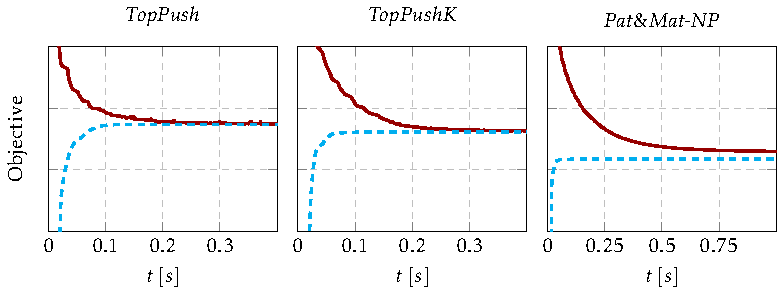
\includegraphics{images/convergence_dual.pdf}
  \caption{Convergence of the objectives for the primal (red line) and dual (blue dashed line) forms with linear kernel.}
  \label{fig: dual convergence}
\end{figure}

\subsection{Primal Formulation: Non-Linear Model}\label{sec: results primal nonlinear}

In this section, we present results for a primal form of formulations from Table~\ref{tab: formulations experiments summary} with a non-linear model. For training, we use the same setting as in Section~\ref{sec: results primal linear}. For MNIST and FashionMNIST datasets, we use a neural network consisting of two convolution layers, followed by a max pooling layer and one fully connected layer of the proper size for binary classification. The rest of the datasets use a similar architecture but with three convolutional layers instead of two. We purposely do not use state-of-the-art architectures since they often lead to a perfect separation of used datasets. Our goal is to show that formulations from Table~\ref{tab: formulations experiments summary} can improve specific metrics such as $\tpratfpr = 0.05$ (when compared to \BaseLine) even with these subpar architectures.

For comparison of all formulations, we use the same two approaches as in Section~\ref{sec: results primal linear}. From Figure~\ref{fig: primal nonlinear CD} and Table~\ref{tab: primal nonlinear medians}, we make several observations:
\begin{itemize}
  \item Most formulations perform well on the criteria for which they are optimized and provide almost perfect separation on MNIST dataset and FashionMNIST dataset.
  \item \DeepTopPush does not provide good results. In fact, the formulation is the worst in five out of six metrics in Figure~\ref{fig: primal nonlinear CD}. However, it can be caused by using relatively large mini-batches concerning the size of the datasets. The true power of the \DeepTopPush is shown in Section~\ref{sec: steganalysis} and~\ref{sec: malware detection}.
  \item \BaseLine formulation performs consistently very well for all metrics. Nevertheless, \BaseLine is the best for neither of the metrics.
  \item \TopPushK(10) fails many times. It is especially evident from Table~\ref{tab: primal nonlinear medians}. \TopPushK(10) achieves 100\% for $\tpratk = 10$ metric for most datasets, which seems as a very good result. However, if we take a look at the~$\auroc$, we can see that the formulation achieves 0\% for the same datasets. The reason for that is simple, \TopPushK(10) assigns the same score to all samples and therefore achieves 100\% true-positive rate but also 100\% false-positive rate.
  \item \PatMatNP formulations provide very good results for all metrics. Moreover, \PatMatNP(0.01) is the best formulation for $\tpratfpr = 0.01,$ and \PatMatNP(0.05) for $\tpratfpr = 0.05.$ It means that both methods are the best for the criterion for which they are optimized. This behavior can also be seen in Table~\ref{tab: primal linear medians}, where \PatMatNP(0.05) is the best formulation for $\tpratfpr = 0.01$ for all datasets.
  \item \tauFPL formulations work well on MNIST and FashinMNIST datasets, but are subpar on the rest.
\end{itemize}

\begin{figure}[!p]
  \centering
  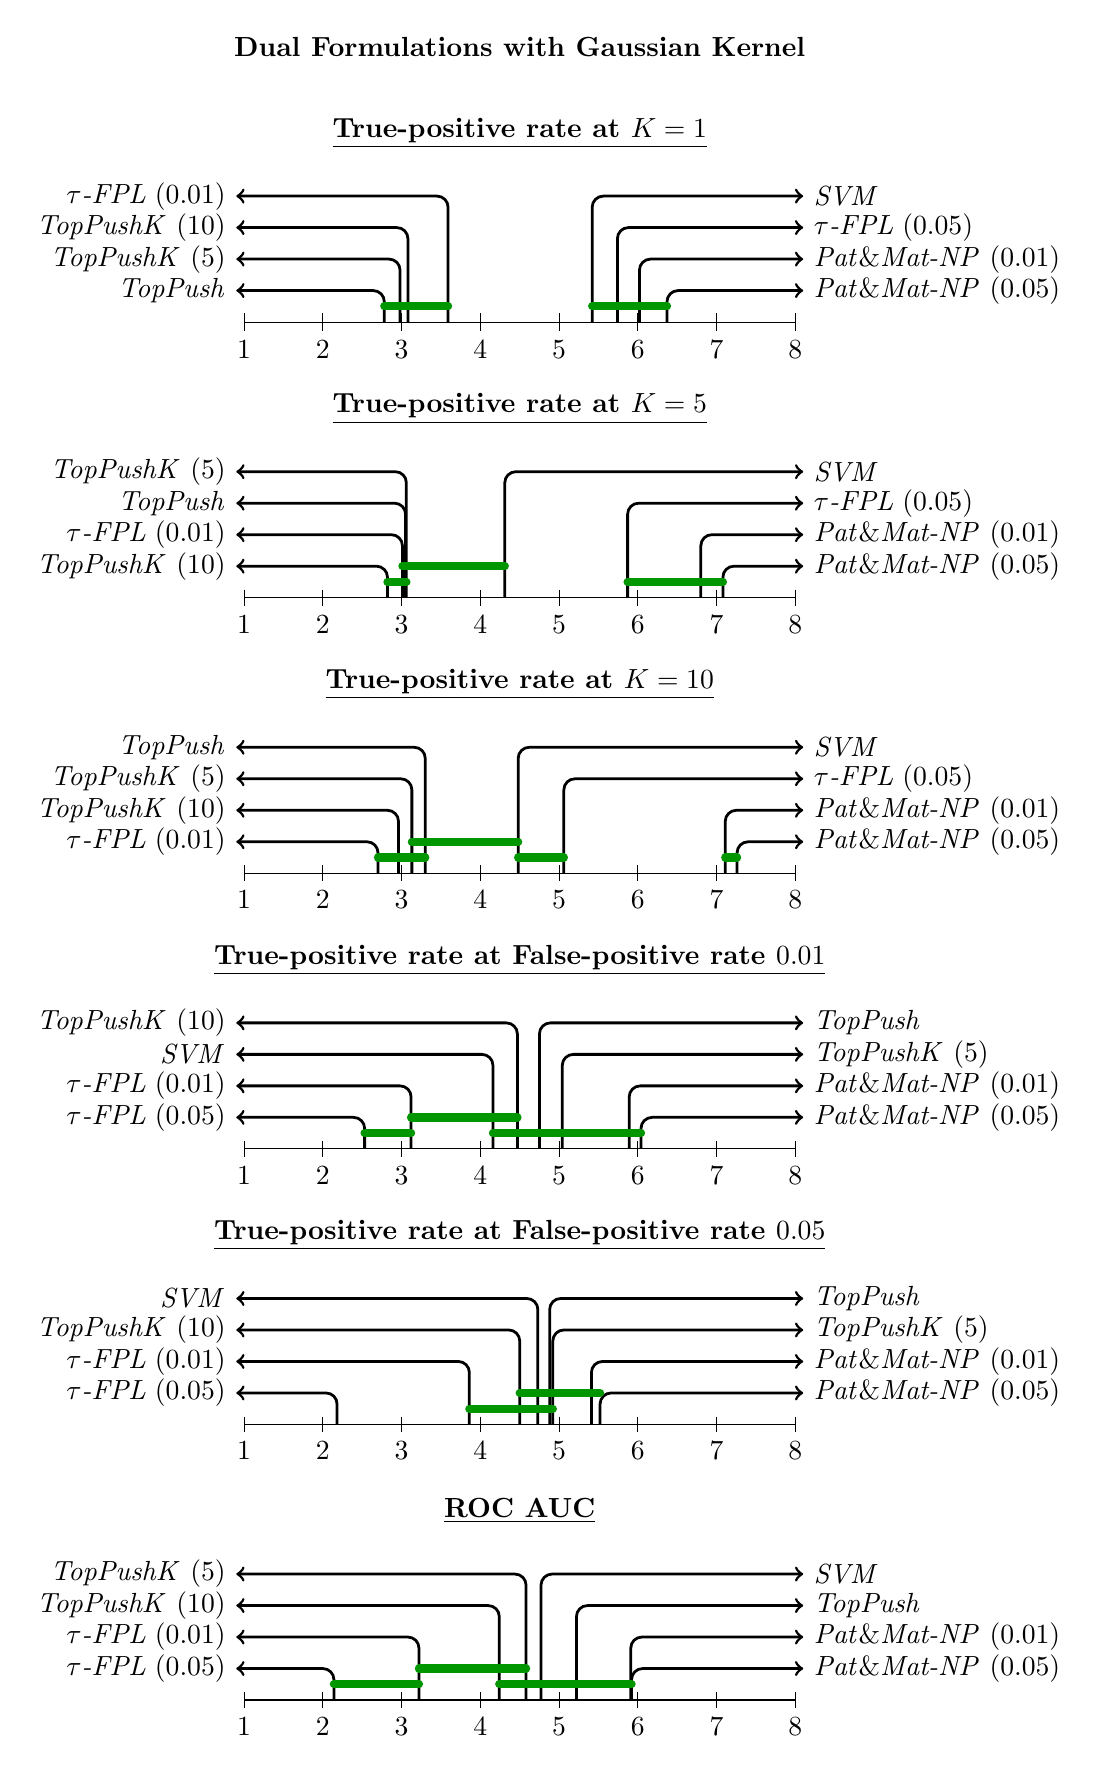
\begin{tikzpicture}  \node at (4.5,2.4) {\textbf{\underline{ROC AUC}}}; 
  \draw (1,0) -- (8,0); 
  \foreach \x in {1,...,8} \draw (\x,0.1) -- (\x,-0.1) node[anchor=north]{$\x$}; 
  \draw[line_node] (2.14,0) -- (2.14,0.4) -- (0.9, 0.4) node[anchor=east] {\tauFPL(0.05)}; 
  \draw[line_node] (3.22,0) -- (3.22,0.8) -- (0.9, 0.8) node[anchor=east] {\tauFPL(0.01)}; 
  \draw[line_node] (4.24,0) -- (4.24,1.2) -- (0.9, 1.2) node[anchor=east] {\TopPushK(10)}; 
  \draw[line_node] (4.58,0) -- (4.58,1.6) -- (0.9, 1.6) node[anchor=east] {\TopPushK(5)}; 
  \draw[line_node] (4.77,0) -- (4.77,1.6) -- (8.1, 1.6) node[anchor=west] {\SVM}; 
  \draw[line_node] (5.22,0) -- (5.22,1.2) -- (8.1, 1.2) node[anchor=west] {\TopPush}; 
  \draw[line_node] (5.91,0) -- (5.91,0.8) -- (8.1, 0.8) node[anchor=west] {\PatMatNP(0.01)}; 
  \draw[line_node] (5.92,0) -- (5.92,0.4) -- (8.1, 0.4) node[anchor=west] {\PatMatNP(0.05)}; 
  \draw[line_cv] (2.14,0.2) -- (3.22, 0.2); 
  \draw[line_cv] (3.22,0.4) -- (4.58, 0.4); 
  \draw[line_cv] (4.24,0.2) -- (5.22, 0.2); 
  \draw[line_cv] (4.58,0.2) -- (5.92, 0.2); 


  \node at (4.5,5.9) {\textbf{\underline{True-positive rate at False-positive rate $0.05$}}}; 
  \draw (1,3.5) -- (8,3.5); 
  \foreach \x in {1,...,8} \draw (\x,3.6) -- (\x,3.4) node[anchor=north]{$\x$}; 
  \draw[line_node] (2.18,3.5) -- (2.18,3.9) -- (0.9, 3.9) node[anchor=east] {\tauFPL(0.05)}; 
  \draw[line_node] (3.86,3.5) -- (3.86,4.3) -- (0.9, 4.3) node[anchor=east] {\tauFPL(0.01)}; 
  \draw[line_node] (4.5,3.5) -- (4.5,4.7) -- (0.9, 4.7) node[anchor=east] {\TopPushK(10)}; 
  \draw[line_node] (4.73,3.5) -- (4.73,5.1) -- (0.9, 5.1) node[anchor=east] {\SVM}; 
  \draw[line_node] (4.88,3.5) -- (4.88,5.1) -- (8.1, 5.1) node[anchor=west] {\TopPush}; 
  \draw[line_node] (4.92,3.5) -- (4.92,4.7) -- (8.1, 4.7) node[anchor=west] {\TopPushK(5)}; 
  \draw[line_node] (5.41,3.5) -- (5.41,4.3) -- (8.1, 4.3) node[anchor=west] {\PatMatNP(0.01)}; 
  \draw[line_node] (5.52,3.5) -- (5.52,3.9) -- (8.1, 3.9) node[anchor=west] {\PatMatNP(0.05)}; 
  \draw[line_cv] (3.86,3.7) -- (4.92, 3.7); 
  \draw[line_cv] (4.5,3.9) -- (5.52, 3.9); 


  \node at (4.5,9.4) {\textbf{\underline{True-positive rate at False-positive rate $0.01$}}}; 
  \draw (1,7.0) -- (8,7.0); 
  \foreach \x in {1,...,8} \draw (\x,7.1) -- (\x,6.9) node[anchor=north]{$\x$}; 
  \draw[line_node] (2.53,7.0) -- (2.53,7.4) -- (0.9, 7.4) node[anchor=east] {\tauFPL(0.05)}; 
  \draw[line_node] (3.12,7.0) -- (3.12,7.8) -- (0.9, 7.8) node[anchor=east] {\tauFPL(0.01)}; 
  \draw[line_node] (4.16,7.0) -- (4.16,8.2) -- (0.9, 8.2) node[anchor=east] {\SVM}; 
  \draw[line_node] (4.47,7.0) -- (4.47,8.6) -- (0.9, 8.6) node[anchor=east] {\TopPushK(10)}; 
  \draw[line_node] (4.75,7.0) -- (4.75,8.6) -- (8.1, 8.6) node[anchor=west] {\TopPush}; 
  \draw[line_node] (5.04,7.0) -- (5.04,8.2) -- (8.1, 8.2) node[anchor=west] {\TopPushK(5)}; 
  \draw[line_node] (5.89,7.0) -- (5.89,7.8) -- (8.1, 7.8) node[anchor=west] {\PatMatNP(0.01)}; 
  \draw[line_node] (6.04,7.0) -- (6.04,7.4) -- (8.1, 7.4) node[anchor=west] {\PatMatNP(0.05)}; 
  \draw[line_cv] (2.53,7.2) -- (3.12, 7.2); 
  \draw[line_cv] (3.12,7.4) -- (4.47, 7.4); 
  \draw[line_cv] (4.16,7.2) -- (5.04, 7.2); 
  \draw[line_cv] (4.75,7.2) -- (6.04, 7.2); 


  \node at (4.5,12.9) {\textbf{\underline{True-positive rate at $K = 10$}}}; 
  \draw (1,10.5) -- (8,10.5); 
  \foreach \x in {1,...,8} \draw (\x,10.6) -- (\x,10.4) node[anchor=north]{$\x$}; 
  \draw[line_node] (2.7,10.5) -- (2.7,10.9) -- (0.9, 10.9) node[anchor=east] {\tauFPL(0.01)}; 
  \draw[line_node] (2.96,10.5) -- (2.96,11.3) -- (0.9, 11.3) node[anchor=east] {\TopPushK(10)}; 
  \draw[line_node] (3.13,10.5) -- (3.13,11.7) -- (0.9, 11.7) node[anchor=east] {\TopPushK(5)}; 
  \draw[line_node] (3.3,10.5) -- (3.3,12.1) -- (0.9, 12.1) node[anchor=east] {\TopPush}; 
  \draw[line_node] (4.48,10.5) -- (4.48,12.1) -- (8.1, 12.1) node[anchor=west] {\SVM}; 
  \draw[line_node] (5.06,10.5) -- (5.06,11.7) -- (8.1, 11.7) node[anchor=west] {\tauFPL(0.05)}; 
  \draw[line_node] (7.11,10.5) -- (7.11,11.3) -- (8.1, 11.3) node[anchor=west] {\PatMatNP(0.01)}; 
  \draw[line_node] (7.26,10.5) -- (7.26,10.9) -- (8.1, 10.9) node[anchor=west] {\PatMatNP(0.05)}; 
  \draw[line_cv] (2.7,10.7) -- (3.3, 10.7); 
  \draw[line_cv] (3.13,10.9) -- (4.48, 10.9); 
  \draw[line_cv] (4.48,10.7) -- (5.06, 10.7); 
  \draw[line_cv] (7.11,10.7) -- (7.26, 10.7); 


  \node at (4.5,16.4) {\textbf{\underline{True-positive rate at $K = 5$}}}; 
  \draw (1,14.0) -- (8,14.0); 
  \foreach \x in {1,...,8} \draw (\x,14.1) -- (\x,13.9) node[anchor=north]{$\x$}; 
  \draw[line_node] (2.82,14.0) -- (2.82,14.4) -- (0.9, 14.4) node[anchor=east] {\TopPushK(10)}; 
  \draw[line_node] (3.01,14.0) -- (3.01,14.8) -- (0.9, 14.8) node[anchor=east] {\tauFPL(0.01)}; 
  \draw[line_node] (3.05,14.0) -- (3.05,15.2) -- (0.9, 15.2) node[anchor=east] {\TopPush}; 
  \draw[line_node] (3.06,14.0) -- (3.06,15.6) -- (0.9, 15.6) node[anchor=east] {\TopPushK(5)}; 
  \draw[line_node] (4.31,14.0) -- (4.31,15.6) -- (8.1, 15.6) node[anchor=west] {\SVM}; 
  \draw[line_node] (5.87,14.0) -- (5.87,15.2) -- (8.1, 15.2) node[anchor=west] {\tauFPL(0.05)}; 
  \draw[line_node] (6.8,14.0) -- (6.8,14.8) -- (8.1, 14.8) node[anchor=west] {\PatMatNP(0.01)}; 
  \draw[line_node] (7.08,14.0) -- (7.08,14.4) -- (8.1, 14.4) node[anchor=west] {\PatMatNP(0.05)}; 
  \draw[line_cv] (2.82,14.2) -- (3.06, 14.2); 
  \draw[line_cv] (3.01,14.4) -- (4.31, 14.4); 
  \draw[line_cv] (5.87,14.2) -- (7.08, 14.2); 


  \node at (4.5,19.9) {\textbf{\underline{True-positive rate at $K = 1$}}}; 
  \draw (1,17.5) -- (8,17.5); 
  \foreach \x in {1,...,8} \draw (\x,17.61) -- (\x,17.39) node[anchor=north]{$\x$}; 
  \draw[line_node] (2.78,17.5) -- (2.78,17.9) -- (0.9, 17.9) node[anchor=east] {\TopPush}; 
  \draw[line_node] (2.98,17.5) -- (2.98,18.3) -- (0.9, 18.3) node[anchor=east] {\TopPushK(5)}; 
  \draw[line_node] (3.08,17.5) -- (3.08,18.7) -- (0.9, 18.7) node[anchor=east] {\TopPushK(10)}; 
  \draw[line_node] (3.59,17.5) -- (3.59,19.1) -- (0.9, 19.1) node[anchor=east] {\tauFPL(0.01)}; 
  \draw[line_node] (5.42,17.5) -- (5.42,19.1) -- (8.1, 19.1) node[anchor=west] {\SVM}; 
  \draw[line_node] (5.74,17.5) -- (5.74,18.7) -- (8.1, 18.7) node[anchor=west] {\tauFPL(0.05)}; 
  \draw[line_node] (6.02,17.5) -- (6.02,18.3) -- (8.1, 18.3) node[anchor=west] {\PatMatNP(0.01)}; 
  \draw[line_node] (6.37,17.5) -- (6.37,17.9) -- (8.1, 17.9) node[anchor=west] {\PatMatNP(0.05)}; 
  \draw[line_cv] (2.78,17.7) -- (3.59, 17.7); 
  \draw[line_cv] (5.42,17.7) -- (6.37, 17.7); 


\node at (4.5, 21.0) {\textbf{Dual Formulations with Gaussian Kernel}}; 
\end{tikzpicture}

  \caption{\textbf{Dual formulations with a gaussian kernel:} Critical difference diagrams (level of importance 0.05) of the Nemenyi post hoc test for the Friedman test. Each diagram shows the mean rank of each method, with rank one being the best. The green horizontal lines group methods with mean ranks that are not significantly different. The critical difference diagrams were computed for mean rank averages over all datasets.}
  \label{fig: dual gauss CD}
\end{figure}

\begin{table}[!p]
  \centering
  \underline{$\tpratk =10$}
  \vspace{0.25cm}\\
  \resizebox{\columnwidth}{!}{% 
    \begin{NiceTabular}{lcccccc}
      \CodeBefore
        \rowcolor{\headercol}{1}
        \rowcolors{3}{\rowcol}{}[restart]
      \Body
      \toprule
      \textbf{Formulation}
        & \textbf{MNIST}
        & \textbf{FashionMNIST}
        & \textbf{CIFAR10}
        & \textbf{CIFAR20}
        & \textbf{CIFAR100}
        & \textbf{SVHN2}\\
      \midrule
      \SVM
        & 97.89
        & \best{95.40}
        & 9.10
        & 4.90
        & \best{11.50}
        & 4.52 \\
      \TopPush
        & 97.62
        & 94.80
        & 10.45
        & \best{6.10}
        & 11.00
        & 5.23 \\
      \TopPushK(5)
        & 97.97
        & 94.90
        & 10.05
        & 6.00
        & 11.0
        & 5.07 \\
      \TopPushK(10)
        & 97.97
        & 94.90
        & 9.85
        & \best{6.10}
        & 11.00
        & 5.18 \\
      \tauFPL(0.01)
        & \best{98.02}
        & 95.05
        & \best{10.70}
        & 5.90
        & 10.5
        & \best{5.25} \\
      \tauFPL(0.05)
        & 92.56
        & \worst{92.20}
        & 10.15
        & 5.10
        & 10.0
        & 5.24 \\
      \PatMatNP(0.01)
        & 88.37
        & 92.50
        & \worst{7.45}
        & 1.40
        & \worst{5.00}
        & \worst{4.02} \\
      \PatMatNP(0.05)
        & \worst{52.60}
        & 92.50
        & \worst{7.45}
        & \worst{1.30}
        & \worst{5.00}
        & 4.05 \\
      \bottomrule
    \end{NiceTabular}
  }
  \vspace{0.25cm}\\
  \underline{$\tpratfpr = 0.05$}
  \vspace{0.25cm}\\
  \resizebox{\columnwidth}{!}{% 
    \begin{NiceTabular}{lcccccc}
      \CodeBefore
        \rowcolor{\headercol}{1}
        \rowcolors{3}{\rowcol}{}[restart]
      \Body
      \toprule
      \textbf{Formulation}
        & \textbf{MNIST}
        & \textbf{FashionMNIST}
        & \textbf{CIFAR10}
        & \textbf{CIFAR20}
        & \textbf{CIFAR100}
        & \textbf{SVHN2}\\
      \midrule
      \SVM
        & 99.74
        & 98.90
        & 60.00
        & \best{44.80}
        & 59.00
        & \worst{59.72} \\
      \TopPush
        & 99.74
        & 98.80
        & 57.10
        & \worst{37.70}
        & 59.50
        & 72.54 \\
      \TopPushK(5)
        & \best{99.82}
        & 98.90
        & 56.25
        & 38.80
        & \worst{57.50}
        & 71.40 \\
      \TopPushK(10)
        & \best{99.82}
        & 98.90
        & 56.90
        & 38.70
        & 58.00
        & 71.61 \\
      \tauFPL(0.01)
        & \best{99.82}
        & 98.90
        & 58.10
        & 39.10
        & 59.00
        & 73.52 \\
      \tauFPL(0.05)
        & 99.74
        & \best{99.10}
        & \best{60.80}
        & 44.40
        & 61.00
        & \best{74.26} \\
      \PatMatNP(0.01)
        & \worst{99.30}
        & \worst{98.10}
        & \worst{54.70}
        & 44.60
        & 62.50
        & 63.47 \\
      \PatMatNP(0.05)
        & 99.38
        & \worst{98.10}
        & \worst{54.70}
        & 44.50
        & \best{63.50}
        & 63.48 \\
      \bottomrule
    \end{NiceTabular}
  }
  \vspace{0.25cm}\\
  \underline{$\auroc$}
  \vspace{0.25cm}\\
  \resizebox{\columnwidth}{!}{% 
    \begin{NiceTabular}{lcccccc}
      \CodeBefore
        \rowcolor{\headercol}{1}
        \rowcolors{3}{\rowcol}{}[restart]
      \Body
      \toprule
      \textbf{Formulation}
        & \textbf{MNIST}
        & \textbf{FashionMNIST}
        & \textbf{CIFAR10}
        & \textbf{CIFAR20}
        & \textbf{CIFAR100}
        & \textbf{SVHN2}\\
      \midrule
      \SVM
        & 99.94
        & 99.66
        & 90.02
        & 79.75
        & 87.80
        & \worst{90.14} \\
      \TopPush
        & 99.94
        & 99.56
        & 89.35
        & 79.06
        & \worst{87.03}
        & 92.77 \\
      \TopPushK(5)
        & 99.95
        & 99.64
        & 89.05
        & 79.13
        & 87.21
        & 92.60 \\
      \TopPushK(10)
        & 99.95
        & 99.67
        & 89.16
        & 79.27
        & 87.78
        & 92.67 \\
      \tauFPL(0.01)
        & \best{99.97}
        & 99.68
        & 89.83
        & 79.07
        & 87.64
        & 92.98 \\
      \tauFPL(0.05)
        & 99.93
        & \best{99.80}
        & \best{90.34}
        & \best{80.17}
        & 88.56
        & \best{93.16} \\
      \PatMatNP(0.01)
        & \worst{99.78}
        & \worst{99.40}
        & 87.62
        & 78.82
        & \best{89.78}
        & 90.80 \\
      \PatMatNP(0.05)
        & \worst{99.78}
        & \worst{99.40}
        & \worst{87.61}
        & \worst{78.76}
        & 89.52
        & 90.82 \\
      \bottomrule
    \end{NiceTabular}
  }
  \caption{\textbf{Dual formulations with a gaussian kernel:} Each table corresponds to one performance metric, and all presented results are medians of ten independent runs for each dataset and formulation pair. The best result for each dataset is highlighted in green, while the worst result is highlighted in red. For better readability, we have reduced the number of discussed metrics compared to Figure~\ref{fig: dual gauss CD}.}
  \label{tab: dual gauss medians}
\end{table}

\begin{figure}[!p]
  \centering
  \documentclass{standalone}
% ------------------------------------------------------------------------------
% Packages
% ------------------------------------------------------------------------------
\usepackage[ddmmyyyy]{datetime}
\usepackage[T1]{fontenc}
\usepackage[utf8]{inputenc}

% Page setting
\usepackage[explicit]{titlesec}
\usepackage{sectsty}
\usepackage{fancyhdr}
\usepackage[title, titletoc]{appendix}

% Fonts
\usepackage{kpfonts}
\usepackage{amsmath}
\usepackage{amssymb}
\usepackage{dsfont}
\usepackage{pifont}

% Graphics and colors
\usepackage{graphicx}
\usepackage{xcolor}
\usepackage{import}

\definecolor{myred}{RGB}{150,0,0}
\definecolor{mygreen}{RGB}{0,150,0}
\definecolor{myblue}{RGB}{0, 101, 189}
\definecolor{myyellow}{RGB}{220, 206, 0}
\definecolor{myorange}{RGB}{255, 153, 51}
\definecolor{mycyan}{RGB}{51, 204, 204}
\definecolor{mypurple}{RGB}{204, 0, 153}

\newcommand{\doccol}{\color{myblue}}

% Hyperrefs
\usepackage[
  pdfusetitle,
  unicode = true,
  bookmarks = true,
  bookmarksnumbered = false,
  bookmarksopen = true,
  breaklinks = false,
  pdfborderstyle = {},
  backref = false,
  colorlinks = true,
  linkcolor = myblue,
  urlcolor = myred,
  citecolor = mygreen,
]{hyperref}


% Captions
\usepackage{caption}

\captionsetup[figure]{position = bottom}
\captionsetup[table]{position = bottom}

% Tables, Algs ...
\usepackage{enumitem}
\usepackage{algorithm}
\usepackage{algorithmicx}
\usepackage{algpseudocode}
\usepackage{booktabs}
\usepackage{nicematrix}

\renewcommand{\arraystretch}{1.5}

\newcommand{\headercol}{myblue!20}
\newcommand{\rowcol}{myblue!10}

% Math
\usepackage{nicefrac}
\usepackage{bm}
\usepackage{thm-restate}
\usepackage{optidef}
\usepackage{xspace}

% Theorems
\usepackage[framemethod=TikZ]{mdframed}
\usepackage{amsthm}
\usepackage{xifthen}

% Tikz and pfgplots
\usepackage{tikz}
\usepackage{pgfplots}
\usepackage{pgfplotstable}

\usetikzlibrary{shapes}
\usetikzlibrary{arrows}
\usetikzlibrary{automata}
\usetikzlibrary{positioning}
\usetikzlibrary{calc}
\usetikzlibrary{intersections}

\pgfplotsset{compat=newest}
\usepgfplotslibrary{groupplots}
\usepgfplotslibrary{fillbetween}

\tikzstyle{line_node} = [line width=1pt, rounded corners, color=black, ->]
\tikzstyle{line_cv} = [line width=3pt, color=mygreen, line cap=round]

% Tmp
\usepackage[color=myred!50]{todonotes}

% ------------------------------------------------------------------------------
% Math declarations
% ------------------------------------------------------------------------------
\newcommand{\Brac}[2][r]{%
  \ifx r#1 \left(       #2 \right)       \else
  \ifx c#1 \left\{      #2 \right\}      \else
  \ifx s#1 \left[       #2 \right]       \else
  \ifx v#1 \left\vert   #2 \right\vert   \else
  \ifx a#1 \left\langle #2 \right\rangle \else
  \ifx t#1 \left\lceil  #2 \right\rceil  \else
  \ifx b#1 \left\lfloor #2 \right\rfloor \else
  \ifx n#1 \left\|      #2 \right\|      \else
  \mathrm{Illegal~option}%
  \fi\fi\fi\fi\fi\fi\fi\fi
}

\newcommand{\clip}[4][s]{
  \ifx s#1 \mathrm{clip}_{\Brac[s]{#2,\; #3}}\Brac{#4} \else
  \ifx u#1 \mathrm{clip}_{\left[#2,\; #3\right)}\Brac{#4} \else
  \ifx l#1 \mathrm{clip}_{\left(#2,\; #3\right]}\Brac{#4} \else
  \mathrm{Illegal~option}%
  \fi\fi\fi
}

\DeclareMathOperator*{\argmax}{arg\,max}

\newcommand{\yesmark}{\textcolor{mygreen}{\ding{51}}}%
\newcommand{\nomark}{\textcolor{myred}{\ding{55}}}
\newcommand{\good}[1]{\textcolor{mygreen}{#1}}
\newcommand{\bad}[1]{\textcolor{myred}{#1}}

\newcommand{\R}{\mathbb{R}}
\newcommand{\N}{\mathbb{N}}
\newcommand{\X}{\mathbb{X}}

\newcommand{\I}{\mathcal{I}}
\newcommand{\Itil}{\tilde{\mathcal{I}}}
\newcommand{\Ineg}{\I_{-}}
\newcommand{\Ipos}{\I_{+}}

\newcommand{\Imb}{\I_{\text{mb}}}
\newcommand{\Imbneg}{\I_{\text{mb},-}}
\newcommand{\Imbpos}{\I_{\text{mb},+}}

\newcommand{\indmax}{j^{\star}}
\newcommand{\indmaxmb}{j^{\star}_{\text{mb}}}

\newcommand{\nall}{n}
\newcommand{\nneg}{n_{-}}
\newcommand{\npos}{n_{+}}
\newcommand{\ntil}{\tilde{n}}

\newcommand{\nmb}{n_{\text{mb}}}
\newcommand{\nmbneg}{n_{\text{mb},-}}
\newcommand{\nmbpos}{n_{\text{mb},+}}

\newcommand{\K}{\mathbb{K}}
\newcommand{\Kall}{\K^{\pm}}
\newcommand{\Kneg}{\K^{-}}

\newcommand{\alphak}{\alpha_{\hat{k}}}
\newcommand{\alphal}{\alpha_{\hat{l}}}
\newcommand{\betak}{\beta_{\hat{k}}}
\newcommand{\betal}{\beta_{\hat{l}}}

\newcommand{\norm}[1]{\Brac[n]{#1}}
\newcommand{\abs}[1]{|#1|}
\newcommand{\inner}[2]{\Brac[a]{#1, \; #2}}
\newcommand{\dd}[1]{\mathop{}\!\mathrm{d}#1}

\newcommand{\Iverson}[1]{\mathds{1}_{\Brac[s]{#1}}}

\newcommand{\EE}{\mathbb{E}}
\newcommand{\PP}{\mathbb{P}}
\newcommand{\bias}{\operatorname{bias}}

\newcommand{\Matrix}[1]{\begin{pmatrix} #1 \end{pmatrix}}
\newcommand{\Set}[2]{\Brac[c]{#1 \; \middle\vert \; #2}}
\newcommand{\domain}{\operatorname*{dom}}

\newcommand{\repeatloop}{\texttt{repeat}\xspace}
\newcommand{\forloop}{\texttt{for}\xspace}

\newcommand{\vecab}{\Matrix{\bm{\alpha} \\ \bm{\beta}}}

% models
\newcommand{\AccatTop}{\emph{Accuracy at the Top}\xspace}
\newcommand{\TopPush}{\emph{TopPush}\xspace}
\newcommand{\TopPushK}{\emph{TopPushK}\xspace}
\newcommand{\tauFPL}{{\emph{$\tau$-FPL}}\xspace}
\newcommand{\TopMeanK}{\emph{TopMeanK}\xspace}
\newcommand{\PatMat}{\emph{Pat}\&\emph{Mat}\xspace}
\newcommand{\PatMatNP}{{\emph{Pat}\&\emph{Mat-NP}}\xspace}
\newcommand{\Grill}{\emph{Grill}\xspace}
\newcommand{\GrillNP}{\emph{Grill-NP}\xspace}
\newcommand{\DeepTopPush}{\emph{DeepTopPush}\xspace}
\newcommand{\TFCO}{\emph{TFCO}\xspace}
\newcommand{\APPerf}{\emph{Ap-Perf}\xspace}
\newcommand{\BaseLine}{\emph{BinCross}\xspace}
\newcommand{\SVM}{\emph{SVM}\xspace}

% counts and rates
\DeclareMathOperator{\tp}{tp}
\DeclareMathOperator{\tn}{tn}
\DeclareMathOperator{\fp}{fp}
\DeclareMathOperator{\fn}{fn}
\DeclareMathOperator{\tpr}{tpr}
\DeclareMathOperator{\tnr}{tnr}
\DeclareMathOperator{\fpr}{fpr}
\DeclareMathOperator{\fnr}{fnr}

\DeclareMathOperator{\tps}{\overline{tp}}
\DeclareMathOperator{\tns}{\overline{tn}}
\DeclareMathOperator{\fps}{\overline{fp}}
\DeclareMathOperator{\fns}{\overline{fn}}

\DeclareMathOperator{\accuracy}{acc}
\DeclareMathOperator{\baccuracy}{bacc}
\DeclareMathOperator{\precision}{precision}
\DeclareMathOperator{\recall}{recall}
\DeclareMathOperator{\pratrec}{Precision@Recall}
\DeclareMathOperator{\postop}{pos@top}

\newcommand{\tpratk}{\operatorname{TPR@}K}
\newcommand{\tpratfpr}{\operatorname{TPR@}\tau}
\newcommand{\auroc}{\operatorname{AUROC}}


% ------------------------------------------------------------------------------
% Document
% ------------------------------------------------------------------------------
\tikzstyle{line_node} = [line width=1pt, rounded corners, color=black, ->]
\tikzstyle{line_cv} = [line width=3pt, color=mygreen, line cap=round]

\begin{document}
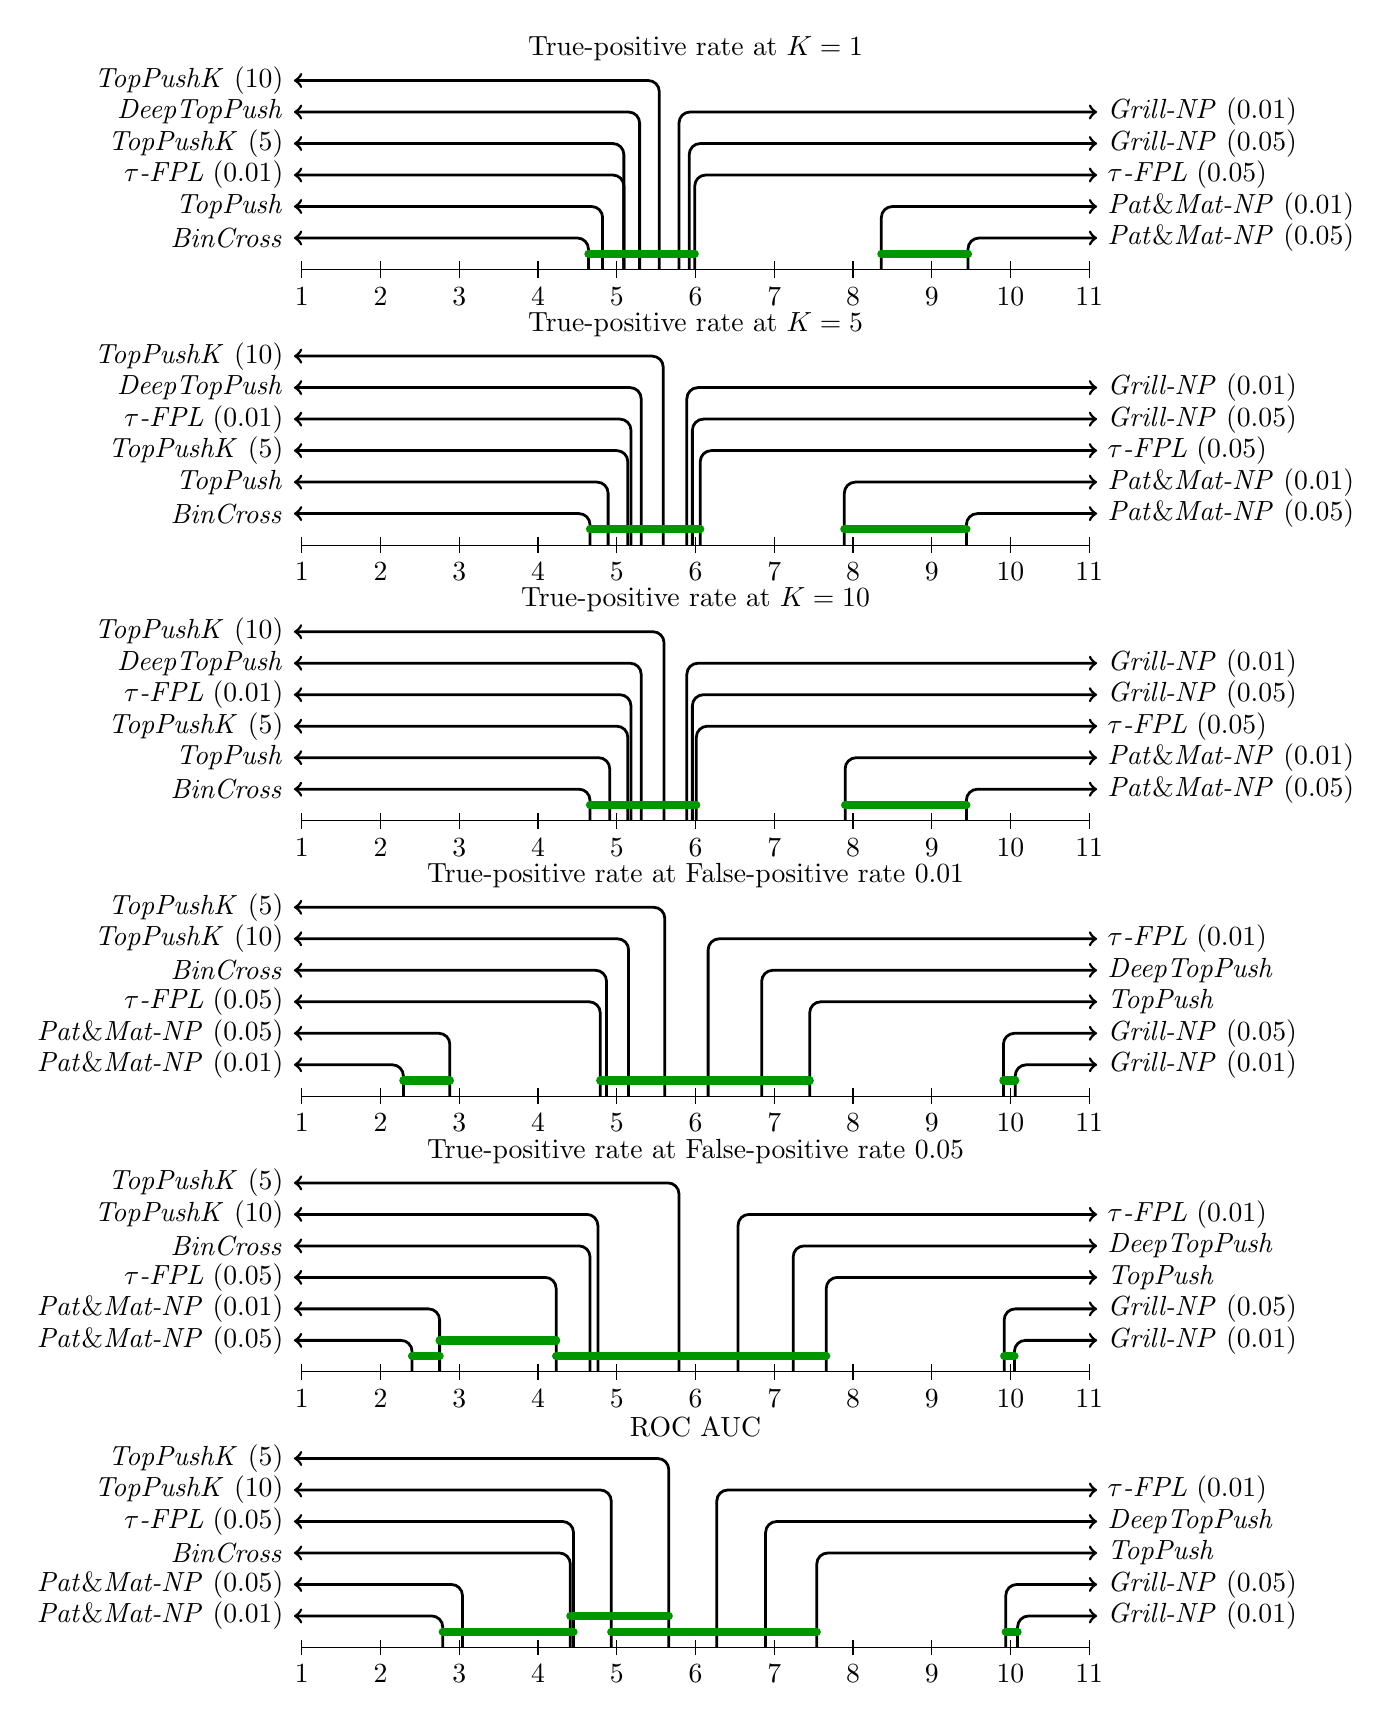
\begin{tikzpicture}
  \node at (6.0,2.8) {ROC AUC}; 
  \draw (1,0) -- (11,0); 
  \foreach \x in {1,...,11} \draw (\x,0.1) -- (\x,-0.1) node[anchor=north]{$\x$}; 
  \draw[line_node] (2.79,0) -- (2.79,0.4) -- (0.9, 0.4) node[anchor=east] {\PatMatNP(0.01)}; 
  \draw[line_node] (3.04,0) -- (3.04,0.8) -- (0.9, 0.8) node[anchor=east] {\PatMatNP(0.05)}; 
  \draw[line_node] (4.41,0) -- (4.41,1.2) -- (0.9, 1.2) node[anchor=east] {\BaseLine}; 
  \draw[line_node] (4.45,0) -- (4.45,1.6) -- (0.9, 1.6) node[anchor=east] {\tauFPL(0.05)}; 
  \draw[line_node] (4.93,0) -- (4.93,2.0) -- (0.9, 2.0) node[anchor=east] {\TopPushK(10)}; 
  \draw[line_node] (5.66,0) -- (5.66,2.4) -- (0.9, 2.4) node[anchor=east] {\TopPushK(5)}; 
  \draw[line_node] (6.27,0) -- (6.27,2.0) -- (11.1, 2.0) node[anchor=west] {\tauFPL(0.01)}; 
  \draw[line_node] (6.89,0) -- (6.89,1.6) -- (11.1, 1.6) node[anchor=west] {\DeepTopPush}; 
  \draw[line_node] (7.54,0) -- (7.54,1.2) -- (11.1, 1.2) node[anchor=west] {\TopPush}; 
  \draw[line_node] (9.94,0) -- (9.94,0.8) -- (11.1, 0.8) node[anchor=west] {\GrillNP(0.05)}; 
  \draw[line_node] (10.09,0) -- (10.09,0.4) -- (11.1, 0.4) node[anchor=west] {\GrillNP(0.01)}; 
  \draw[line_cv] (2.79,0.2) -- (4.45, 0.2); 
  \draw[line_cv] (4.41,0.4) -- (5.66, 0.4); 
  \draw[line_cv] (4.93,0.2) -- (6.27, 0.2); 
  \draw[line_cv] (5.66,0.2) -- (6.89, 0.2); 
  \draw[line_cv] (6.27,0.2) -- (7.54, 0.2); 
  \draw[line_cv] (9.94,0.2) -- (10.09, 0.2); 

  \node at (6.0,6.3) {True-positive rate at False-positive rate $0.05$}; 
  \draw (1,3.5) -- (11,3.5); 
  \foreach \x in {1,...,11} \draw (\x,3.6) -- (\x,3.4) node[anchor=north]{$\x$}; 
  \draw[line_node] (2.4,3.5) -- (2.4,3.9) -- (0.9, 3.9) node[anchor=east] {\PatMatNP(0.05)}; 
  \draw[line_node] (2.75,3.5) -- (2.75,4.3) -- (0.9, 4.3) node[anchor=east] {\PatMatNP(0.01)}; 
  \draw[line_node] (4.23,3.5) -- (4.23,4.7) -- (0.9, 4.7) node[anchor=east] {\tauFPL(0.05)}; 
  \draw[line_node] (4.66,3.5) -- (4.66,5.1) -- (0.9, 5.1) node[anchor=east] {\BaseLine}; 
  \draw[line_node] (4.76,3.5) -- (4.76,5.5) -- (0.9, 5.5) node[anchor=east] {\TopPushK(10)}; 
  \draw[line_node] (5.79,3.5) -- (5.79,5.9) -- (0.9, 5.9) node[anchor=east] {\TopPushK(5)}; 
  \draw[line_node] (6.54,3.5) -- (6.54,5.5) -- (11.1, 5.5) node[anchor=west] {\tauFPL(0.01)}; 
  \draw[line_node] (7.24,3.5) -- (7.24,5.1) -- (11.1, 5.1) node[anchor=west] {\DeepTopPush}; 
  \draw[line_node] (7.66,3.5) -- (7.66,4.7) -- (11.1, 4.7) node[anchor=west] {\TopPush}; 
  \draw[line_node] (9.92,3.5) -- (9.92,4.3) -- (11.1, 4.3) node[anchor=west] {\GrillNP(0.05)}; 
  \draw[line_node] (10.05,3.5) -- (10.05,3.9) -- (11.1, 3.9) node[anchor=west] {\GrillNP(0.01)}; 
  \draw[line_cv] (2.4,3.7) -- (2.75, 3.7); 
  \draw[line_cv] (2.75,3.9) -- (4.23, 3.9); 
  \draw[line_cv] (4.23,3.7) -- (5.79, 3.7); 
  \draw[line_cv] (4.76,3.7) -- (6.54, 3.7); 
  \draw[line_cv] (5.79,3.7) -- (7.24, 3.7); 
  \draw[line_cv] (6.54,3.7) -- (7.66, 3.7); 
  \draw[line_cv] (9.92,3.7) -- (10.05, 3.7); 

  \node at (6.0,9.8) {True-positive rate at False-positive rate $0.01$}; 
  \draw (1,7.0) -- (11,7.0); 
  \foreach \x in {1,...,11} \draw (\x,7.1) -- (\x,6.9) node[anchor=north]{$\x$}; 
  \draw[line_node] (2.29,7.0) -- (2.29,7.4) -- (0.9, 7.4) node[anchor=east] {\PatMatNP(0.01)}; 
  \draw[line_node] (2.88,7.0) -- (2.88,7.8) -- (0.9, 7.8) node[anchor=east] {\PatMatNP(0.05)}; 
  \draw[line_node] (4.79,7.0) -- (4.79,8.2) -- (0.9, 8.2) node[anchor=east] {\tauFPL(0.05)}; 
  \draw[line_node] (4.87,7.0) -- (4.87,8.6) -- (0.9, 8.6) node[anchor=east] {\BaseLine}; 
  \draw[line_node] (5.15,7.0) -- (5.15,9.0) -- (0.9, 9.0) node[anchor=east] {\TopPushK(10)}; 
  \draw[line_node] (5.61,7.0) -- (5.61,9.4) -- (0.9, 9.4) node[anchor=east] {\TopPushK(5)}; 
  \draw[line_node] (6.16,7.0) -- (6.16,9.0) -- (11.1, 9.0) node[anchor=west] {\tauFPL(0.01)}; 
  \draw[line_node] (6.84,7.0) -- (6.84,8.6) -- (11.1, 8.6) node[anchor=west] {\DeepTopPush}; 
  \draw[line_node] (7.45,7.0) -- (7.45,8.2) -- (11.1, 8.2) node[anchor=west] {\TopPush}; 
  \draw[line_node] (9.91,7.0) -- (9.91,7.8) -- (11.1, 7.8) node[anchor=west] {\GrillNP(0.05)}; 
  \draw[line_node] (10.06,7.0) -- (10.06,7.4) -- (11.1, 7.4) node[anchor=west] {\GrillNP(0.01)}; 
  \draw[line_cv] (2.29,7.2) -- (2.88, 7.2); 
  \draw[line_cv] (4.79,7.2) -- (6.16, 7.2); 
  \draw[line_cv] (5.15,7.2) -- (6.84, 7.2); 
  \draw[line_cv] (6.16,7.2) -- (7.45, 7.2); 
  \draw[line_cv] (9.91,7.2) -- (10.06, 7.2); 

  \node at (6.0,13.3) {True-positive rate at $K = 10$}; 
  \draw (1,10.5) -- (11,10.5); 
  \foreach \x in {1,...,11} \draw (\x,10.6) -- (\x,10.4) node[anchor=north]{$\x$}; 
  \draw[line_node] (4.66,10.5) -- (4.66,10.9) -- (0.9, 10.9) node[anchor=east] {\BaseLine}; 
  \draw[line_node] (4.91,10.5) -- (4.91,11.3) -- (0.9, 11.3) node[anchor=east] {\TopPush}; 
  \draw[line_node] (5.14,10.5) -- (5.14,11.7) -- (0.9, 11.7) node[anchor=east] {\TopPushK(5)}; 
  \draw[line_node] (5.18,10.5) -- (5.18,12.1) -- (0.9, 12.1) node[anchor=east] {\tauFPL(0.01)}; 
  \draw[line_node] (5.31,10.5) -- (5.31,12.5) -- (0.9, 12.5) node[anchor=east] {\DeepTopPush}; 
  \draw[line_node] (5.6,10.5) -- (5.6,12.9) -- (0.9, 12.9) node[anchor=east] {\TopPushK(10)}; 
  \draw[line_node] (5.89,10.5) -- (5.89,12.5) -- (11.1, 12.5) node[anchor=west] {\GrillNP(0.01)}; 
  \draw[line_node] (5.96,10.5) -- (5.96,12.1) -- (11.1, 12.1) node[anchor=west] {\GrillNP(0.05)}; 
  \draw[line_node] (6.01,10.5) -- (6.01,11.7) -- (11.1, 11.7) node[anchor=west] {\tauFPL(0.05)}; 
  \draw[line_node] (7.9,10.5) -- (7.9,11.3) -- (11.1, 11.3) node[anchor=west] {\PatMatNP(0.01)}; 
  \draw[line_node] (9.44,10.5) -- (9.44,10.9) -- (11.1, 10.9) node[anchor=west] {\PatMatNP(0.05)}; 
  \draw[line_cv] (4.66,10.7) -- (6.01, 10.7); 
  \draw[line_cv] (7.9,10.7) -- (9.44, 10.7); 

  \node at (6.0,16.8) {True-positive rate at $K = 5$}; 
  \draw (1,14.0) -- (11,14.0); 
  \foreach \x in {1,...,11} \draw (\x,14.1) -- (\x,13.9) node[anchor=north]{$\x$}; 
  \draw[line_node] (4.66,14.0) -- (4.66,14.4) -- (0.9, 14.4) node[anchor=east] {\BaseLine}; 
  \draw[line_node] (4.89,14.0) -- (4.89,14.8) -- (0.9, 14.8) node[anchor=east] {\TopPush}; 
  \draw[line_node] (5.14,14.0) -- (5.14,15.2) -- (0.9, 15.2) node[anchor=east] {\TopPushK(5)}; 
  \draw[line_node] (5.18,14.0) -- (5.18,15.6) -- (0.9, 15.6) node[anchor=east] {\tauFPL(0.01)}; 
  \draw[line_node] (5.31,14.0) -- (5.31,16.0) -- (0.9, 16.0) node[anchor=east] {\DeepTopPush}; 
  \draw[line_node] (5.59,14.0) -- (5.59,16.4) -- (0.9, 16.4) node[anchor=east] {\TopPushK(10)}; 
  \draw[line_node] (5.89,14.0) -- (5.89,16.0) -- (11.1, 16.0) node[anchor=west] {\GrillNP(0.01)}; 
  \draw[line_node] (5.96,14.0) -- (5.96,15.6) -- (11.1, 15.6) node[anchor=west] {\GrillNP(0.05)}; 
  \draw[line_node] (6.06,14.0) -- (6.06,15.2) -- (11.1, 15.2) node[anchor=west] {\tauFPL(0.05)}; 
  \draw[line_node] (7.89,14.0) -- (7.89,14.8) -- (11.1, 14.8) node[anchor=west] {\PatMatNP(0.01)}; 
  \draw[line_node] (9.44,14.0) -- (9.44,14.4) -- (11.1, 14.4) node[anchor=west] {\PatMatNP(0.05)}; 
  \draw[line_cv] (4.66,14.2) -- (6.06, 14.2); 
  \draw[line_cv] (7.89,14.2) -- (9.44, 14.2); 

  \node at (6.0,20.3) {True-positive rate at $K = 1$}; 
  \draw (1,17.5) -- (11,17.5); 
  \foreach \x in {1,...,11} \draw (\x,17.61) -- (\x,17.39) node[anchor=north]{$\x$}; 
  \draw[line_node] (4.64,17.5) -- (4.64,17.9) -- (0.9, 17.9) node[anchor=east] {\BaseLine}; 
  \draw[line_node] (4.82,17.5) -- (4.82,18.3) -- (0.9, 18.3) node[anchor=east] {\TopPush}; 
  \draw[line_node] (5.09,17.5) -- (5.09,18.7) -- (0.9, 18.7) node[anchor=east] {\tauFPL(0.01)}; 
  \draw[line_node] (5.09,17.5) -- (5.09,19.1) -- (0.9, 19.1) node[anchor=east] {\TopPushK(5)}; 
  \draw[line_node] (5.29,17.5) -- (5.29,19.5) -- (0.9, 19.5) node[anchor=east] {\DeepTopPush}; 
  \draw[line_node] (5.54,17.5) -- (5.54,19.9) -- (0.9, 19.9) node[anchor=east] {\TopPushK(10)}; 
  \draw[line_node] (5.79,17.5) -- (5.79,19.5) -- (11.1, 19.5) node[anchor=west] {\GrillNP(0.01)}; 
  \draw[line_node] (5.92,17.5) -- (5.92,19.1) -- (11.1, 19.1) node[anchor=west] {\GrillNP(0.05)}; 
  \draw[line_node] (5.99,17.5) -- (5.99,18.7) -- (11.1, 18.7) node[anchor=west] {\tauFPL(0.05)}; 
  \draw[line_node] (8.36,17.5) -- (8.36,18.3) -- (11.1, 18.3) node[anchor=west] {\PatMatNP(0.01)}; 
  \draw[line_node] (9.46,17.5) -- (9.46,17.9) -- (11.1, 17.9) node[anchor=west] {\PatMatNP(0.05)}; 
  \draw[line_cv] (4.64,17.7) -- (5.99, 17.7); 
  \draw[line_cv] (8.36,17.7) -- (9.46, 17.7); 
\end{tikzpicture}
\end{document}

  \caption{\textbf{Primal formulations with a non-linear model:} Critical difference diagrams (level of importance 0.05) of the Nemenyi post hoc test for the Friedman test. Each diagram shows the mean rank of each method, with rank one being the best. The green horizontal lines group methods with mean ranks that are not significantly different. The critical difference diagrams were computed for mean rank averages over all datasets.}
  \label{fig: primal nonlinear CD}
\end{figure}

\begin{table}[!p]
  \centering
  \underline{$\tpratk =10$}
  \vspace{0.25cm}\\
  \resizebox{\columnwidth}{!}{% 
    \begin{NiceTabular}{lccccccc}
      \CodeBefore
        \rowcolor{\headercol}{1}
        \rowcolors{3}{\rowcol}{}[restart]
      \Body
      \toprule
      \textbf{Formulation}
        & \textbf{MNIST}
        & \textbf{FashionMNIST}
        & \textbf{CIFAR10}
        & \textbf{CIFAR20}
        & \textbf{CIFAR100}
        & \textbf{SVHN2}
        & \textbf{SVHN2Extra}\\
      \midrule
      \BaseLine
        & \best{99.26}
        & \best{98.10}
        & 11.40
        & 3.50
        & 5.00
        & 11.34
        & 15.95 \\
      \DeepTopPush
        & 98.42
        & 97.60
        & \worst{0.20}
        & 0.20
        & \worst{0.00}
        & \worst{0.17}
        & \worst{0.00} \\
      \TopPushK(5)
        & 98.54
        & 97.50
        & 2.00
        & \worst{0.00}
        & 8.50
        & 10.58
        & 16.12 \\
      \TopPushK(10)
        & 98.24
        & 96.90
        & 12.55
        & \best{100.00}
        & \best{100.00}
        & \best{100.00}
        & \best{100.00} \\
      \tauFPL(0.01)
        & 98.72
        & 97.50
        & 1.00
        & 0.20
        & 9.00
        & 9.52
        & \worst{0.00} \\
      \tauFPL(0.05)
        & 96.78
        & 96.50
        & 14.80
        & 0.30
        & 8.50
        & 13.05
        & 12.48 \\
      \PatMatNP(0.01)
        & 98.54
        & 97.45
        & \best{32.45}
        & 4.80
        & 20.00
        & 13.92
        & 19.33 \\
      \PatMatNP(0.05)
        & \worst{82.86}
        & \worst{94.30}
        & 26.55
        & 5.90
        & 11.50
        & 11.36
        & 15.98 \\
      \bottomrule
    \end{NiceTabular}
  }
  \vspace{0.25cm}\\
  \underline{$\tpratfpr = 0.05$}
  \vspace{0.25cm}\\
  \resizebox{\columnwidth}{!}{% 
    \begin{NiceTabular}{lccccccc}
      \CodeBefore
        \rowcolor{\headercol}{1}
        \rowcolors{3}{\rowcol}{}[restart]
      \Body
      \toprule
      \textbf{Formulation}
        & \textbf{MNIST}
        & \textbf{FashionMNIST}
        & \textbf{CIFAR10}
        & \textbf{CIFAR20}
        & \textbf{CIFAR100}
        & \textbf{SVHN2}
        & \textbf{SVHN2Extra}\\
      \midrule
      \BaseLine
        & \best{100.00}
        & \best{99.90}
        & 83.35
        & 48.00
        & 82.00
        & 94.66
        & 97.71 \\
      \DeepTopPush
        & \worst{99.82}
        & \worst{99.70}
        & \worst{5.85}
        & 8.90
        & 9.00
        & 40.14
        & \worst{0.00} \\
      \TopPushK(5)
        & \best{100.00}
        & 99.85
        & 34.30
        & 7.70
        & 53.50
        & 86.54
        & 93.96 \\
      \TopPushK(10)
        & \best{100.00}
        & \best{99.90}
        & 27.95
        & \worst{0.00}
        & \worst{0.00}
        & \worst{0.00}
        & \worst{0.00} \\
      \tauFPL(0.01)
        & \best{100.00}
        & \best{99.90}
        & 24.40
        & 11.50
        & 65.50
        & 87.60
        & \worst{0.00} \\
      \tauFPL(0.05)
        & \best{100.00}
        & \best{99.90}
        & 82.75
        & 18.00
        & 66.50
        & 94.51
        & 97.52 \\
      \PatMatNP(0.01)
        & \best{100.00}
        & \best{99.90}
        & 91.55
        & 52.20
        & 79.00
        & 95.49
        & 98.43 \\
      \PatMatNP(0.05)
        & \best{100.00}
        & \best{99.90}
        & \best{91.75}
        & \best{57.70}
        & \best{85.00}
        & \best{95.53}
        & \best{98.50} \\
      \bottomrule
    \end{NiceTabular}
  }
  \vspace{0.25cm}\\
  \underline{$\auroc$}
  \vspace{0.25cm}\\
  \resizebox{\columnwidth}{!}{% 
    \begin{NiceTabular}{lccccccc}
      \CodeBefore
        \rowcolor{\headercol}{1}
        \rowcolors{3}{\rowcol}{}[restart]
      \Body
      \toprule
      \textbf{Formulation}
        & \textbf{MNIST}
        & \textbf{FashionMNIST}
        & \textbf{CIFAR10}
        & \textbf{CIFAR20}
        & \textbf{CIFAR100}
        & \textbf{SVHN2}
        & \textbf{SVHN2Extra}\\
      \midrule
      \BaseLine
        & \best{100.00}
        & \best{99.98}
        & 96.85
        & 84.67
        & 95.94
        & 98.54
        & 99.20 \\
      \DeepTopPush
        & 99.98
        & \worst{99.95}
        & \worst{49.51}
        & 59.40
        & 56.68
        & 83.12
        & 1.61 \\
      \TopPushK(5)
        & \best{100.0}
        & 99.97
        & 77.10
        & 55.50
        & 84.24
        & 96.57
        & 98.32 \\
      \TopPushK(10)
        & \best{100.00}
        & \best{99.98}
        & 74.26
        & \worst{0.00}
        & \worst{0.00}
        & \worst{0.00}
        & \worst{0.00} \\
      \tauFPL(0.01)
        & \best{100.0}
        & \best{99.98}
        & 70.96
        & 60.03
        & 90.16
        & 96.68
        & 25.84 \\
      \tauFPL(0.05)
        & 99.99
        & 99.97
        & 95.86
        & 68.18
        & 90.76
        & 98.50
        & 99.12 \\
      \PatMatNP(0.01)
        & 99.99
        & \best{99.98}
        & 97.90
        & 84.38
        & 93.84
        & 98.74
        & \best{99.38} \\
      \PatMatNP(0.05)
        & \worst{99.96}
        & 99.96
        & \best{98.24}
        & \best{88.39}
        & \best{96.56}
        & \best{98.76}
        & 99.32 \\
      \bottomrule
    \end{NiceTabular}
  }
  \caption{\textbf{Primal formulations with a non-linear model:} Each table corresponds to one performance metric, and all presented results are medians of ten independent runs for each dataset and formulation pair. The best result for each dataset is highlighted in green, while the worst result is highlighted in red. For better readability, we have reduced the number of discussed metrics compared to Figure~\ref{fig: primal nonlinear CD}.}
  \label{tab: primal nonlinear medians}
\end{table}

\pagebreak

\section{Steganalysis}\label{sec: steganalysis}

In the previous section, we presented results on standard image recognition datasets. Even though the results are quite good, they did not fully show the importance of the problem of classification at the top. To show the importance of this problem properly,  we need to find the field where the maximizing true-positive rate at the low false-positive rate is an important task. Such a field can be, for example, steganalysis.

The standard way to share secret information these days is through encryption. However, in such a case, the presence of a secret message (even though encrypted) is obvious. Steganography aims to hide the fact that communication is taking place by hiding the secret message within an ordinary file (usually called a cover file) to avoid detection. The secret message is then extracted at its destination. The secret data can be hidden in almost any type of digital content. However, the most popular are images. There are two reasons for this. The first of them is the ubiquity of images on the Internet and, therefore, the ease of using them as cover files for secret messages. The second reason is their large potential payload, i.e., it is possible to hide a lot of information in high-resolution images. With an appropriate cover image and steganography tools, it is possible to create a stego-image (image with a hidden message) that can not be recognized from the cover image by human perception. However, each tool leaves a fingerprint or signature in the image that can be used to detect stego images. The field that tries to detect stego images and possibly decrypt messages from them is called steganalysis. In steganalysis, the goal is to achieve the best true-positive rate with the lowest possible false-positive rate. Therefore steganalysis is the domain suitable for the problem of classification at the top.~\cite{morkel2005overview, silman2001steganography} 

For the experiments, we use two private steganography datasets. Both these datasets are created from the same database of cover images comprising approximately 450 000 images from Flickr. All these images are in JPEG format with a quality factor of 80. The datasets used for the experiments differ in the algorithm that was used to generate the stego images. The stego images for the first dataset were generated using the \textbf{Nsf5} algorithm~\cite{fridrich2007statistically}, while the stego images for the second dataset were generated using the \textbf{JMiPOD} algorithm~\cite{cogranne2020steganography}. For simplicity, we have named the datasets according to the stego algorithms used.

\subsection{Nsf5}

As we mentioned before, the stego images in the first dataset were generated using the \textbf{Nsf5} algorithm~\cite{fridrich2007statistically} using the payload 0.2. Since generating stego images is expensive, only 10\% of all cover images are used to generate their stego counterparts. Moreover, the dataset does not contain images but 22 500 features extracted using the CC-JRM algorithm~\cite{kodovsky2012steganalysis}. Finally, the whole dataset is divided into train/validation/test sets in the 0.45/0.05/0.5 ratio. The resulting sizes of the splits, as well as the number of stego samples in them, are summarized in Table~\ref{tab: datasets summary}. 

Since the resulting classification task is relatively easy to solve, we decided to use a simple linear model. The number of training samples and their size is not too large. Therefore we can load the whole dataset into memory. It allows us to use full gradient descent instead of its stochastic version. As an optimizer, we use the ADAM~\cite{kingma2014adam} with default settings and fixed step length~$\alpha = 0.01.$ We also fix the number of epochs to 1000 for all formulations. Finally, we repeat each experiment ten times with ten different random seeds.

Figure~\ref{fig: steganalysis nsf5} shows ROC curves for the test set of \textbf{Nsf5} dataset. For simplicity, we show ROC curves only for one experiment run. Moreover, Table~\ref{tab: steganalysis nsf5} shows seven different performance metrics computed for each formulation. Each shown result in this table is a median of ten independent runs. \BaseLine provides inferior results for all metrics. The best and worst results are highlighted in green and red. Surprisingly, \BaseLine performs the worst even for the $\auroc.$ On the other hand, \DeepTopPush excels at very low false-positive rates, as seen from the table and the figure. In fact, \DeepTopPush provides the best results for four out of seven performance metrics. Note that all these four metrics operate at extremely low false-positive rates. We can also see that \PatMatNP($10^{-5}$) is the best at false-positive rate~$10^{-4}$. This is probably caused by the approximation of the true top $\tau$-quantile of all scores of negative samples used in \PatMatNP formulation. Therefore, \PatMatNP($10^{-5}$) is optimized for a false-positive rate slightly higher than~$10^{-5}$ and as a consequence outperforms \PatMatNP($10^{-4}$) at false-positive rate~$10^{-4}$. Similar behavior can be seen for \PatMatNP($10^{-4}$) and \PatMatNP($10^{-3}$) at false-positive rate~$10^{-3}$.

\begin{figure}
  \centering
  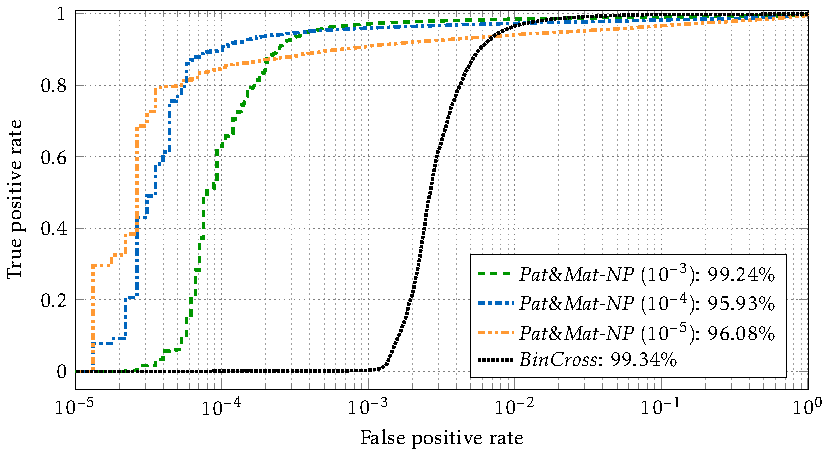
\includegraphics{images/stego_nsft5.pdf}
  \caption{\textbf{Nsf5 dataset:} ROC curves with logarithmic $x$-axis.}
  \label{fig: steganalysis nsf5}
\end{figure}

\begin{table}[!t]
  \centering
  \begin{NiceTabular}{lccccccc}
    \CodeBefore
    \rowcolor{\headercol}{1-2}
    \rowcolors{4}{\rowcol}{}[restart]
    \Body
    \toprule
    \Block[c]{2-1}{\textbf{Formulation}}
    & \Block[c]{2-1}{$\auroc$}
    & \Block[c]{1-3}{$\tpratk$}
    &&& \Block[c]{1-3}{$\tpratfpr$} \\
    \cline{3-8}
    && $1$
    & $10$
    & $5$
    & $10^{-5}$
    & $10^{-4}$
    & $10^{-3}$ \\
    \midrule
    \BaseLine
    & \worst{95.84}
    & \worst{0.0}
    & \worst{0.0}
    & \worst{0.0}
    & \worst{0.0}
    & \worst{0.02}
    & \worst{0.7} \\
    \DeepTopPush
    & 98.29
    & \best{5.07}
    & \best{35.48}
    & \best{57.66}
    & \best{48.65}
    & 89.56
    & 93.67 \\
    \PatMatNP($10^{-5}$)
    & 98.81
    & 2.55
    & 23.02
    & 47.24
    & 35.28
    & \best{91.9}
    & 95.84 \\
    \PatMatNP($10^{-4}$)
    & 98.98
    & \worst{0.0}
    & 0.05
    & 4.34
    & 1.78
    & 79.76
    & \best{96.18} \\
    \PatMatNP($10^{-3}$)
    & \best{99.26}
    & \worst{0.0}
    & \worst{0.0}
    & 0.01
    & \worst{0.0}
    & 0.29
    & 91.98 \\
    \bottomrule
  \end{NiceTabular}
  \caption{\textbf{NSF5 dataset:} All presented results are medians of ten independent runs with different random seeds. Each column of the table corresponds to one performance metric, and every row to one formulation. The best result for each metric is highlighted in green, while the worst is highlighted in red.}
  \label{tab: steganalysis nsf5}
\end{table}

\subsection{JMiPOD}

The second dataset was created in a different way. Firstly only images that can be cropped to size $256 \times 256$ were used. All such images were cropped losslessly using \emph{jpegtran} library~\cite{libjpeg2014} and the stego images were generated using the JMiPOD algorithm~\cite{cogranne2020steganography} using payload 0.1. As in the case of Nsf5 dataset, only 10\% of all cover images are used to generate their stego counterparts. Unlike the Nsf5 dataset, \textbf{JMiPOD} dataset contains images and not features extracted from them. The entire dataset is divided into train/validation/test sets in the 0.375/0.125/0.5 ratio. The resulting sizes of the splits and the number of stego images in them are summarized in Table~\ref{tab: datasets summary}. 

In this case, the resulting classification task is quite complicated. Therefore we decided to use pre-trained EfficientNet-B0~\cite{tan2019efficientnet} as the model. Originally the model was trained for 1000 classes. Therefore, we removed the last fully-connected layer and replaced it with a randomly initialized fully-connected layer of appropriate size for binary classification. The resulting model is large, and it is not possible to use a full gradient. For this reason, we use stochastic gradient descent with balanced mini-batches of size 256. As an optimizer, we use the ADAM~\cite{kingma2014adam} with default settings and fixed step length~$\alpha = 0.01.$ Finally, we fix the number of epochs to 30 for all formulations, and we repeat each experiment ten times with different random seeds.

\begin{figure}[!t]
  \centering
  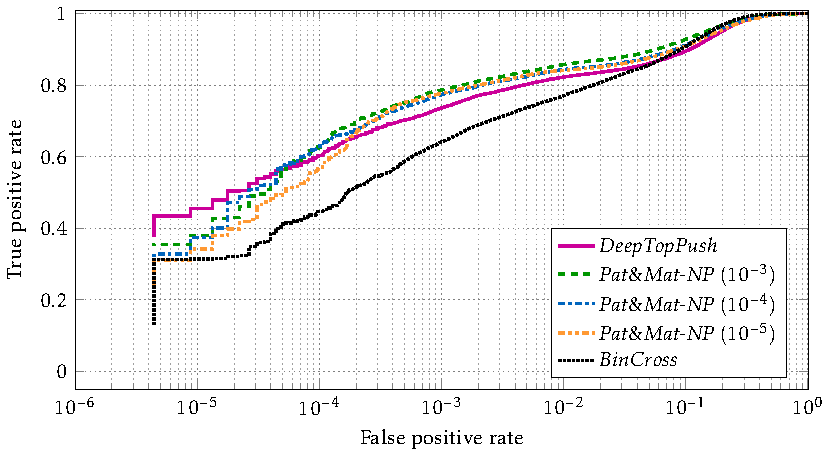
\includegraphics{images/stego_jmipod.pdf}
  \caption{\textbf{JMiPOD dataset:} ROC curves with logarithmic $x$-axis.}
  \label{fig: steganalysis jmipod}
\end{figure}

\begin{table}[!t]
  \centering
  \begin{NiceTabular}{lccccccc}
    \CodeBefore
      \rowcolor{\headercol}{1-2}
      \rowcolors{4}{\rowcol}{}[restart]
    \Body
    \toprule
    \Block[c]{2-1}{\textbf{Formulation}}
      & \Block[c]{2-1}{$\auroc$}
      & \Block[c]{1-3}{$\tpratk$}
      &&& \Block[c]{1-3}{$\tpratfpr$} \\
    \cline{3-8}
      && $1$
      & $10$
      & $5$
      & $10^{-5}$
      & $10^{-4}$
      & $10^{-3}$ \\
    \midrule
    \BaseLine
      & 97.5
      & \worst{13.52}
      & \worst{24.65}
      & \worst{29.54}
      & \worst{27.28}
      & \worst{44.58}
      & \worst{63.84} \\
    \DeepTopPush
      & \worst{97.26}
      & \best{34.25}
      & \best{42.57}
      & \best{47.3}
      & \best{43.59}
      & 60.42
      & 73.67 \\
    \PatMatNP($10^{-4}$)
      & 97.49
      & 25.66
      & 36.76
      & 45.19
      & 38.28
      & 63.49
      & 77.43 \\
    \PatMatNP($10^{-3}$)
      & \best{98.0}
      & 26.99
      & 38.76
      & 44.83
      & 42.17
      & \best{64.5}
      & \best{78.11} \\
    \bottomrule
  \end{NiceTabular}
  \caption{\textbf{JMiPOD dataset:} All presented results are medians of ten independent runs with different random seeds. Each column of the table corresponds to one performance metric, and every row to one formulation. The best result for each metric is highlighted in green, while the worst is highlighted in red.}
  \label{tab: steganalysis jmipod}
\end{table}

Figure~\ref{fig: steganalysis jmipod} shows ROC curves for the test set of \textbf{JMiPOD} dataset. Moreover, Table~\ref{tab: steganalysis jmipod} shows seven performance metrics. Each shown result in this table is a median of ten independent runs. The best and worst results are highlighted in green and red. Since trained models use stochastic gradient descent, the results are not as evident as for the Nsf5 dataset. \BaseLine still provides the worst results for most metrics, but the differences are much smaller than for the Nsf5 dataset. We can see that \DeepTopPush again provides the best performance for four of the seven metrics. It shows that the enhanced minibatch used in \DeepTopPush Algorithm~\ref{alg: deep toppush} improves the approximation quality of the true threshold and reduces the bias of the sampled gradient (as we already showed in Figure~\ref{fig:thresholds2}). Even though \PatMatNP($10^{-3}$) and \PatMatNP($10^{-4}$) were trained for different levels of false-positive rate, they both perform similarly. As we said before, the decision threshold~$t$ of \PatMatNP model approximates the true top $\tau$-quantile of all scores of negative samples. Since we use mini-batches with 128 negative samples, the smallest quantile that can be found on this minibatch is~$\tau = \frac{1}{128} \approx 0.0078.$ If we try to approximate smaller quantiles, we always get the same results. Therefore, \PatMatNP($10^{-3}$) and \PatMatNP($10^{-4}$) should work almost identically, and we can see from both the figure and the table, that these two formulations provide similar results. For this reason we omit \PatMatNP($10^{-5}$) in this experiment.

\section{Malware Detection}\label{sec: malware detection}

In the previous section, we presented results from the domain of steganalysis. Another domain in which formulations from the presented framework can be very useful is the domain of malware detection. As an example, consider standard antivirus software on a personal computer. Every user wants to be protected, so the goal of antivirus software is to detect as much malware as possible. However, if the antivirus is too restrictive, it can easily happen that clean software is marked as malware, i.e., the antivirus can easily produce false alarms. If the antivirus produces false alarms too often, it can negatively affect the user experience and may lead to uninstalling the antivirus completely. Therefore, the goal of every antivirus is to maximize a true-positive rate at a very low false-positive rate, which is precisely what the formulations from the framework do.

In this section, we present results on a real-world dataset provided by a renowned cybersecurity company. The dataset consists of malware analysis reports of executable files. The dataset is extremely tough as individual samples are JSON files whose size ranges from 1kB to 2.5MB. The sample structure is highly complicated because each sample has a different number of features, and features may have a complicated structure, such as a list of ports to which the file connects. This contrasts sharply with standard datasets, where each sample has the same number of features, and each feature is a real number. The usual approach to processing such complicated data is to manually create feature vectors and use them for training instead of the original data. However, such an approach is extremely time-demanding and requires expert knowledge of the original data. For this reason, we decided to use a different approach called Hierarchical Multiple Instance Learning (HMIL)~\cite{pevny2017using}. For the training, we use a publicly available implementation of HMIL~\cite{mandlik2021mill}, which allows training models directly from JSON files without requiring complicated feature extraction.

Due to the immense dataset size (see Table~\ref{tab: datasets summary}), we train each formulation only once. Moreover, we use only the formulations that worked the best in the previous experiments, i.e., we use only the \BaseLine, \PatMatNP($10^{-2}$), \PatMatNP($10^{-3}$) and \DeepTopPush. As an optimizer, we use the ADAM~\cite{kingma2014adam} with default settings and fixed step length~$\alpha = 0.01.$ We also use balanced mini-batches of size 2000, which allows us to obtain a very good estimate of the true thresholds as discussed in Section~\ref{sec: biased threshold estimate}. Finally, we fix the number of epochs to 100 for all formulations.

Figure~\ref{fig: malware detection} shows the ROC curves for all formulations. It is clear that \DeepTopPush is the best at low false-positive rates. Even at the extremely low false positive rate $\tau=10^{-5}$, \DeepTopPush correctly identified $46\%$ of malware. We can also see that \PatMatNP($10^{-3}$) is the best at false-positive rate~$10^{-3}$, which is exactly the point for which the formulation should be optimized. However, at this false-positive rate, \DeepTopPush performs almost as well as \PatMatNP($10^{-3}$). Finally, all formulations perform equally well at the false-positive rate~$10^{-2}$.

\begin{figure}
  \centering
  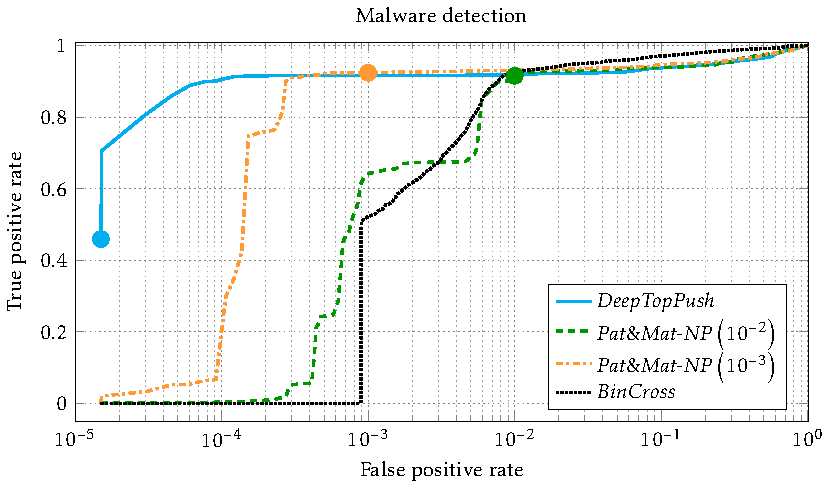
\includegraphics{images/malware_detection.pdf}
  \caption{\textbf{Malware detection:} ROC curves with logarithmic $x$-axis.}
  \label{fig: malware detection}
\end{figure}
\hfill
